\documentclass[12pt]{article}
\usepackage{amsmath}
\usepackage{tikz-dependency}
\DeclareMathOperator*{\argmax}{arg\,max}
\DeclareMathOperator*{\argmin}{arg\,min}
\DeclareMathOperator{\E}{\mathop{\mathbb{E}}}


\usepackage{longtable}


\usepackage{natbib}

\usepackage{hyperref}

\usepackage{amssymb}% http://ctan.org/pkg/amssymb
\usepackage{pifont}% http://ctan.org/pkg/pifont
\newcommand{\cmark}{\ding{51}}%
\newcommand{\xmark}{\ding{55}}%

\usepackage[english]{babel}
\usepackage[utf8]{inputenc}
\usepackage{bm}
\usepackage{graphicx}
\usepackage{tikz}
\usepackage{xcolor}
\usepackage{url}
\usepackage{rotating}
\usepackage{multirow}
\usepackage{natbib}
\usepackage{arydshln}

\newcommand{\key}[1]{\textbf{#1}}





\usepackage{mathtools}
\DeclarePairedDelimiter{\ceiling}{\lceil}{\rceil}

\title{Supplemental Materials for ``Universals of word order result from optimization of grammars for efficient communication''}
\author{
        Michael Hahn \\
                Department of Linguistics\\
       Stanford University
            \and
       Daniel Jurafsky\\
       Department of Linguistics\\
       Stanford University \\
       \and
       Richard Futrell\\
       Department of Language Science\\
       University of California, Irvine
}
\date{\today}

\begin{document}
\maketitle

\section{Formalization of Correlations}

Here we describe how we selected the correlations in Table 1 of the main paper, and how we formalized these using syntactic relations defined by Universal Dependencies.

We base our formalization on the comprehensive study by Dryer \cite{dryer1992greenbergian}.\footnote{Regarding recent objections by~\cite{dunn2011evolved}, see follow-ups by \cite{levy2011computational}, and \cite{croft2011greenbergian}.}
Greenberg's original study was based on 30 languages; more recently, Dryer \cite{dryer1992greenbergian} documented the word order correlations based on typological data from 625 languages.
\cite{dryer1992greenbergian} formulated these universals as correlations between the order of objects and verbs and the orders of other syntactic relations.
We test our ordering grammars for these correlations by testing whether the coefficients for these syntactic relations have the same sign as the coefficient of the verb-object relation.
Testing correlations is therefore constrained by the degree to which these relations are annotated in UD.
The verb-object relation corresponds to the  \emph{obj} relation defined by UD.
While most of the other relations also correspond to UD relations, some are not annotated reliably.
We were able formalize eleven out of Dryer's seventeen correlations in UD.
Six of these could not be expressed individually in UD, and were collapsed into three coarse-grained correlations:
First, tense/aspect and negative auxiliaries are together represented by the \emph{aux} relation in UD.
Second, the relation between complementizers and adverbial subordinators with their complement clauses is represented by the \emph{lifted\_mark} relation.
Third, we both the verb-PP relation and the relation between adjectives and their standard of comparison is captured by the \emph{obl} relation.


We excluded three correlations that are not annotated reliably in UD, and are only relevant to some of the world's languages: Question particles, plural words (i.e., independent plural markers), and articles.
All three types of elements occur at most in parts of the 51 UD languages, and none of them is annotated reliably in those languages where they occur.
Among these three types of elements, the one most prominent in our sample of 51 languages is articles (occurring in many European languages); UD subsumes them under the \emph{det} relation, which is also used for other frequent elements, such as demonstratives and quantifiers.

We also excluded the verb-manner adverb correlation.
UD does not distinguish manner adverbs from other elements labeled as adverbs, such as sentence-level adverbs and negation markers, whose ordering is very different from manner adverbs.
All types of adverbs are unified under the \emph{advmod} relation.
In the real orderings in our sample of 51 UD languages, the dominant ordering of \emph{advmod} almost always matches that of subjects -- that is, \emph{advmod} dependents are ordered after the verb only in VSO languages.
This ordering behavior is very different from that documented for manner adverbs by Dryer.



We further excluded the verb-subject correlation, which is not satisfied by much more than half of the world's languages (51 \% among those with annotation in \cite{wals-81}, with clear violation in 35.4 \%).
It is satisfied only in 33\% of our sample of 51 UD languages, as quantified using the grammars we extracted.
Dryer \cite{dryer1992greenbergian} counts this as a correlation since he describes the distribution of subject order as an interaction between a weak correlation with object order, and a very strong dominance principle favoring SV orderings.
We focus on the modeling of correlations, and leave dominance principles to future research.
We therefore excluded this correlation here.
%We note that efficiency makes predictions compatible with the pattern observed in our sample of 51 languages, potentially in line with the noisy-channel explanation of SVO described by~\cite{gibson2013noisy} (see Table~\ref{tab:all-predictions}).

The resulting operationalization is shown in Table~\ref{table:greenberg-dryer}.

\begin{table*}[ht]
	\begin{center}
\begin{tabular}{|ll|l|l|}
	\hline
	\multicolumn{2}{|c|}{Correlates with...}   &          \multirow{2}{*}{Operationalization}   & \multirow{2}{*}{\cite{greenberg1963universals}}    \\ 
	verb & object &    \\ \hline \hline % \textsc{verb} $\xrightarrow{obj}$ \textsc{noun}
%adp. &
adposition    &    NP    &    case   & 3, 4   \\ \hline
copula  verb  &    predicate    &    cop   & --    \\\hline
`want'    &    VP    &    xcomp   & 15   \\\hline
tense/aspect auxiliary    &    VP    &    \multirow{2}{*}{aux}   & 16, 13  \\
	negative auxiliary    &    VP    &    & -- \\ \hline
complementizer    &    S    &   \multirow{2}{*}{mark}  & --    \\
	adverbial subordinator & S &  & -- \\ \hline
noun    &    genitive    &    nmod & 2, 23   \\ \hline
noun    &    relative clause    &    acl   &  24    \\ \hline
	adjective & standard of comparison & \multirow{2}{*}{obl} & --\\
verb    &    PP    &    & 22   \\
 \hline
%comp. &
%\multirow{3}{*}{NP}&
%	AP &
    \multicolumn{3}{l}{\footnotesize{Significance levels: $^*$: $p < 0.05$, $^{**}$: $p < 0.01$, $^{***}$: $p < 0.001$}}
\end{tabular}
	\end{center}
	\caption{Greenbergian Correlations according to Dryer \cite{dryer1992greenbergian}, with operationalizations with Universal Dependencies. We also provide the corresponding numbers in Greenberg's original study.}\label{table:greenberg-dryer}
\end{table*}



%croft2011greenbergian
%dryer2011evidence

\section{Supporting Analyses for Study 1}

\paragraph{Other tests, maybe som viz}

\paragraph{Pareto Curve}

It has to be convex, so don't need to do more.

\section{Results on all UD Relations}
Table~\ref{tab:all-predictions} shows the predicted prevalence of correlations between the \emph{obj} dependency and all UD dependency types, along with the expected prevalence according to typological studies.

We also report results for grammars optimized for predictability and parseability individually.

Further, we report results for grammars optimized for dependency length minimization (DLM).
DLM can be seen as a heuristic approximation to efficiency.
We also found that DLM is predicted by efficiency optimization.
Indeed, we show that optimizing for DLM makes predictions similar to efficiency optimization.

\begin{table*} % TODO figure out away to make this table more aesthetic
	\begin{center}
	
\small{
\begin{tabular}{|l|l|l|ll|l|l|}
	\hline
	Relation & Real & DepL & Pred & Pars & Efficiency & Expected Prevalence  \\ \hline
% From Dryer	
acl  &  80   &   \textbf{85}$^{***}$   &   43   &   \textbf{82}$^{***}$   &   \textbf{71}$^{***}$  & $>50\%$  \citep{dryer1992greenbergian} \\
aux  &  12   &   \textbf{26}$^{***}$   &   \textbf{19}$^{***}$   &   49   &   \textbf{35}$^{**}$  & $<50\%$ \citep{dryer1992greenbergian} \\
lifted\_case  &  86   &   \textbf{81}$^{***}$   &   \textbf{40}$^{**}$   &   \textbf{77}$^{***}$   &   \textbf{67}$^{***}$ & $> 50 \%$ \citep{dryer1992greenbergian}  \\
lifted\_cop  &  94   &   \textbf{80}$^{***}$   &   59   &   \textbf{72}$^{***}$   &   \textbf{63}$^{**}$  & $> 50 \%$ \citep{dryer1992greenbergian} \\
lifted\_mark  &  76   &   \textbf{85}$^{***}$   &   \textbf{57}$^{*}$   &   \textbf{76}$^{***}$   &   \textbf{72}$^{***}$  & $> 50 \%$ \citep{dryer1992greenbergian} \\
nmod  &  80   &   \textbf{82}$^{***}$   &   49   &   \textbf{71}$^{***}$   &   \textbf{68}$^{***}$  & $> 50 \%$ \citep{dryer1992greenbergian} \\ 
obl  &  88   &   \textbf{78}$^{***}$   &   \textbf{71}$^{***}$   &   46   &   \textbf{68}$^{***}$  &  $> 50 \%$ \citep{dryer1992greenbergian} \\
xcomp  &  88   &   \textbf{90}$^{***}$   &   \textbf{76}$^{***}$   &   \textbf{89}$^{***}$   &   \textbf{85}$^{***}$  &  $> 50 \%$ \citep{dryer1992greenbergian} \\
\hdashline
nsubj  &  33   &   \textbf{29}$^{***}$   &   53   &   \textbf{7}$^{***}$   &   \textbf{23}$^{***}$  & $> 50 \%$ \citep{dryer1992greenbergian} \\

\hline
% Other universals, not in Dryer
advcl  &  86   &   \textbf{84}$^{***}$   &   51   &   \textbf{67}$^{***}$   &   \textbf{67}$^{*}$  & $>50\%$ \citep{greenberg1963universals,diessel2001ordering} \\
ccomp  &  86   &   \textbf{88}$^{***}$   &   \textbf{70}$^{**}$   &   \textbf{77}$^{***}$   &   \textbf{77}$^{**}$ & $>50\%$ (cf. \cite{dryer1980positional}) \\ % TODO According to Dryer 1980, there is a correlation
csubj  &  79   &   \textbf{78}$^{***}$   &   60   &   \textbf{66}$^{***}$   &   \textbf{68}$^{**}$  & $>50\%$ (cf. \cite{dryer1980positional}) \\% TODO According to Dryer 1980, there is a correlation
amod  &  51   &   \textbf{84}$^{***}$   &   42   &   \textbf{53}$^{*}$   &   51   & $\approx 50\%$ \citep{dryer1992greenbergian} \\
nummod  &  37   &   \textbf{74}$^{**}$   &   49   &   52   &   52 & $\approx 50\%$ \citep[][89A, 83A]{wals} \\ % 

\hline
% Typological data not available
appos  &  77   &   \textbf{77}$^{***}$   &   49   &   \textbf{67}$^{***}$   &   \textbf{62}$^{**}$ &  Unknown \\%($>50\%$? correlates with \textit{nmod} according to Greenberg U 23)  \\ % \cite{cinque2009greenberg} claims it correlates with OV/VO. However, it's not clear to me how closely appos matches the subject of the typological claim
lifted\_cc  &  71   &   \textbf{83}$^{***}$   &   51   &   \textbf{81}$^{***}$   &   \textbf{71}$^{***}$  & Unknown \\
expl  &  12   &   36   &   62   &   40   &   53  & Unknown \\
iobj  &  74   &   49   &   \textbf{78}$^{***}$   &   \textbf{38}$^{*}$   &   62  & Unknown \\
vocative  &  46   &   \textbf{42}$^{*}$   &   59   &   45   &   \textbf{45}$^{*}$  & Unknown \\

\hline
% Uninterpretable
compound  &  66   &   \textbf{61}$^{*}$   &   48   &   \textbf{58}$^{*}$   &   52  & Uninterpretable \\
det  &  31   &   \textbf{71}$^{***}$   &   \textbf{56}$^{*}$   &   48   &   54  & Uninterpretable \\%$.50\%$ for articles, $\approx 50\%$ for others, \citep{dryer1992greenbergian} \\
dislocated  &  47   &   61   &   \textbf{68}$^{**}$   &   55   &   58  & Uninterpretable \\
dep  &  56   &   \textbf{64}$^{*}$   &   52   &   58   &   \textbf{58}$^{*}$   & Uninterpretable \\
advmod  &  35   &   51   &   \textbf{18}$^{***}$   &   47   &   \textbf{39}$^{**}$  & Uninterpretable \\

\hline
% UD artifacts
conj  &  72   &   \textbf{82}$^{***}$   &   \textbf{42}$^{**}$   &   \textbf{62}$^{***}$   &   \textbf{59}$^{*}$  & UD artifact  \\
discourse  &  24   &   \textbf{36}$^{**}$   &   \textbf{41}$^{*}$   &   49   &   46  & UD artifact   \\
fixed  &  78   &   \textbf{32}$^{***}$   &   45   &   47   &   44  & UD artifact   \\
flat  &  73   &   \textbf{66}$^{**}$   &   45   &   \textbf{59}$^{**}$   &   54  & UD artifact   \\
goeswith  &  61   &   57   &   44   &   57   &   52  & UD artifact   \\
list  &  94   &   59   &   50   &   54   &   52  & UD artifact  \\
orphan  &  82   &   \textbf{70}$^{**}$   &   50   &   \textbf{55}$^{*}$   &   59  & UD artifact   \\
parataxis  &  66   &   56   &   43   &   57   &   59  & UD artifact  \\
reparandum  &  18   &   53   &   57   &   43   &   48  & UD artifact  \\


 \hline
%comp. &
%\multirow{3}{*}{NP}&
%	AP &
    \multicolumn{7}{l}{\footnotesize{Significance levels: $^*$: $p < 0.05$, $^{**}$: $p < 0.01$, $^{***}$: $p < 0.001$}}
\end{tabular}
}

\end{center}
\caption{Predictions on all UD relations occurring in more than one language. Numbers are the fraction of languages where the direction of the given relation agrees in direction with the \emph{obj} relation. In the last column, we indicate what direction would be expected typologically. The first section correspond to universals from Dryer. ``Uninterpretable'' UD relations are those which collapse so many different linguistic relationships that they are not linguistically meaningful. ``UD artifact'' relations are those whose order is determined strictly by UD parsing standards, such that their order is not linguistically meaningful: these include dependencies such as the connection between two parts of a word that have been separated by whitespace inserted as a typo (\emph{goeswith}).}
\label{tab:all-predictions}
\end{table*}


\section{Posterior}

\begin{figure}
	\begin{center}
	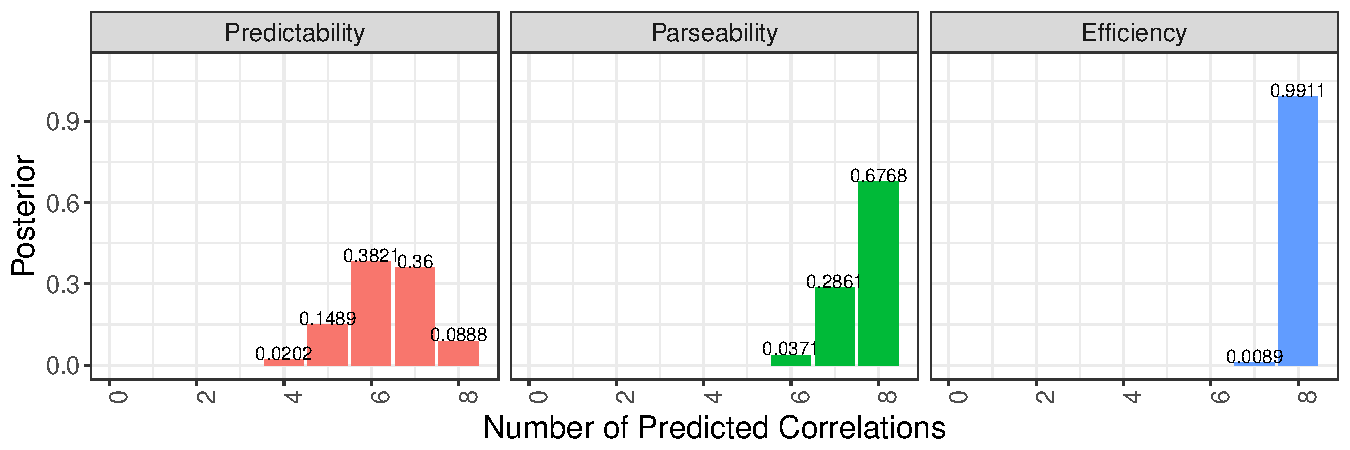
\includegraphics[width=0.48\textwidth]{../results/correlations/figures/posterior-satisfied-universals-together-large-three.pdf}
	\end{center}
	\caption{Posterior of the number of correlations correctly predicted by efficiency and its components, in a Bayesian multivariate mixed-effects logistic regression with random effects for languages and language families.}\label{fig:posterior}
\end{figure}



\begin{table*}
	\begin{center}
%		\setlength\tabcolsep{1.5pt}
\begin{tabular}{c|ll|c|c|cc|ccccccccccc}
	\hline
	%&
	&	\multicolumn{2}{|c|}{Correlates with...}   &         \multirow{2}{*}{Real}   &  \multirow{2}{*}{Efficiency} &  \multirow{2}{*}{Predictability} &  \multirow{2}{*}{Parseability} & \\ 
	&	verb & object     & & &   \\ 
	&	\emph{wrote} & \emph{letters} & & & \\ \hline \hline % \textsc{verb} $\xrightarrow{obj}$ \textsc{noun}
	\multirow{2}{*}{\raisebox{.5pt}{\textcircled{\raisebox{-.9pt} {1}}}}	&	adposition    &    NP       
				&   \multirow{2}{*}{  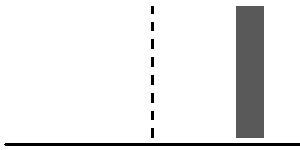
\includegraphics[width=0.06\textwidth]{../results/correlations/figures/posteriors/posterior_Real_lifted_case.pdf}     } 
		&   \multirow{2}{*}{  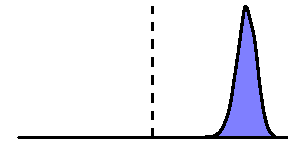
\includegraphics[width=0.06\textwidth]{../results/correlations/figures/posteriors/posterior_Efficiency_lifted_case.pdf}     }
		&   \multirow{2}{*}{  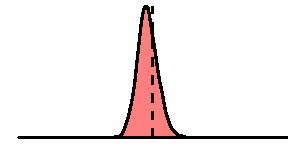
\includegraphics[width=0.06\textwidth]{../results/correlations/figures/posteriors/posterior_Predictability_lifted_case.pdf}     } 
		&   \multirow{2}{*}{  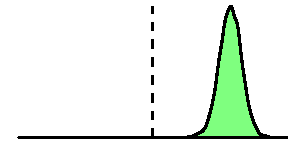
\includegraphics[width=0.06\textwidth]{../results/correlations/figures/posteriors/posterior_Parseability_lifted_case.pdf}     }  & \\
	&		\emph{to}            & \emph{a friend} &&&\\ \hline
	\multirow{2}{*}{\raisebox{.5pt}{\textcircled{\raisebox{-.9pt} {2}}}}	&copula    &    NP         
		&   \multirow{2}{*}{  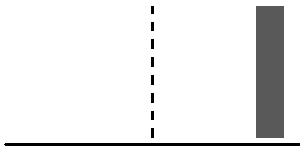
\includegraphics[width=0.06\textwidth]{../results/correlations/figures/posteriors/posterior_Real_lifted_cop.pdf}     } 
		&   \multirow{2}{*}{  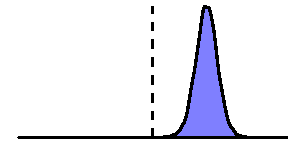
\includegraphics[width=0.06\textwidth]{../results/correlations/figures/posteriors/posterior_Efficiency_lifted_cop.pdf}     } 
		&   \multirow{2}{*}{  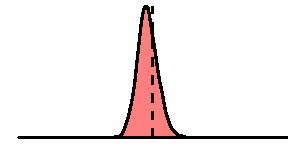
\includegraphics[width=0.06\textwidth]{../results/correlations/figures/posteriors/posterior_Predictability_lifted_case.pdf}     }
	&   \multirow{2}{*}{  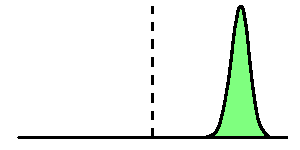
\includegraphics[width=0.06\textwidth]{../results/correlations/figures/posteriors/posterior_Parseability_lifted_cop.pdf}     } 
& \\
	&	\emph{is}        & \emph{a friend}  &&&\\ \hline
	\multirow{2}{*}{\raisebox{.5pt}{\textcircled{\raisebox{-.9pt} {3}}}}	&auxiliary    &    VP       
		&   \multirow{2}{*}{  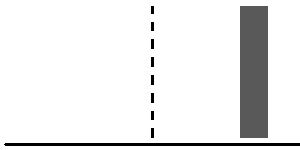
\includegraphics[width=0.06\textwidth]{../results/correlations/figures/posteriors/posterior_Real_aux.pdf}     } 
	&   \multirow{2}{*}{  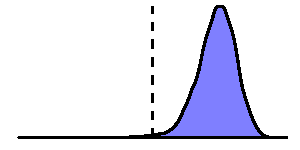
\includegraphics[width=0.06\textwidth]{../results/correlations/figures/posteriors/posterior_Efficiency_aux.pdf}     } 
	&   \multirow{2}{*}{  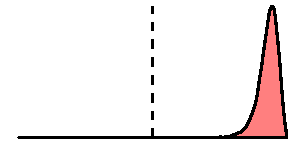
\includegraphics[width=0.06\textwidth]{../results/correlations/figures/posteriors/posterior_Predictability_aux.pdf}     } 
		&   \multirow{2}{*}{  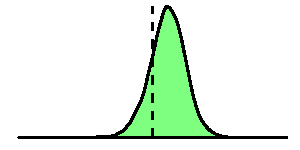
\includegraphics[width=0.06\textwidth]{../results/correlations/figures/posteriors/posterior_Parseability_aux.pdf}     } & \\
	&	\emph{has}          & \emph{written}  &&&\\ \hline
	\multirow{2}{*}{\raisebox{.5pt}{\textcircled{\raisebox{-.9pt} {4}}}}	&noun    &    genitive      
		&   \multirow{2}{*}{  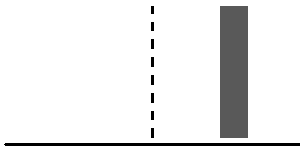
\includegraphics[width=0.06\textwidth]{../results/correlations/figures/posteriors/posterior_Real_nmod.pdf}     } 
	&   \multirow{2}{*}{  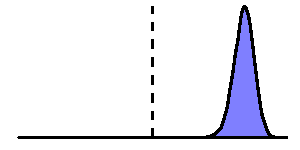
\includegraphics[width=0.06\textwidth]{../results/correlations/figures/posteriors/posterior_Efficiency_nmod.pdf}     } 
	&   \multirow{2}{*}{  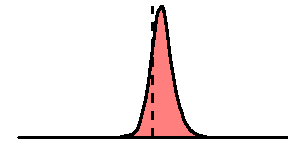
\includegraphics[width=0.06\textwidth]{../results/correlations/figures/posteriors/posterior_Predictability_nmod.pdf}     } 
		&   \multirow{2}{*}{  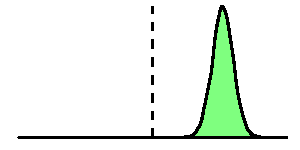
\includegraphics[width=0.06\textwidth]{../results/correlations/figures/posteriors/posterior_Parseability_nmod.pdf}     } & \\
	&	\emph{friend} &  \emph{of John}  &&&\\ \hline
	\multirow{2}{*}{\raisebox{.5pt}{\textcircled{\raisebox{-.9pt} {5}}}}	&noun    &    relative clause      
		&   \multirow{2}{*}{  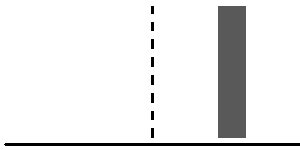
\includegraphics[width=0.06\textwidth]{../results/correlations/figures/posteriors/posterior_Real_acl.pdf}     } 
	&   \multirow{2}{*}{  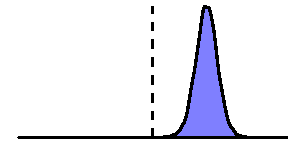
\includegraphics[width=0.06\textwidth]{../results/correlations/figures/posteriors/posterior_Efficiency_lifted_cop.pdf}     }
	&   \multirow{2}{*}{  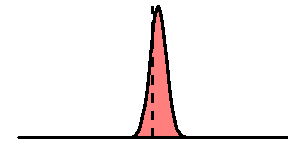
\includegraphics[width=0.06\textwidth]{../results/correlations/figures/posteriors/posterior_Predictability_lifted_cop.pdf}     }
		&   \multirow{2}{*}{  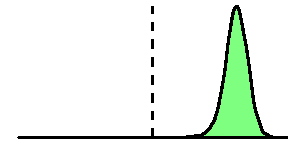
\includegraphics[width=0.06\textwidth]{../results/correlations/figures/posteriors/posterior_Parseability_acl.pdf}     } & \\
	&	\emph{books} & \emph{that you read}  &&&\\ \hline
	\multirow{2}{*}{\raisebox{.5pt}{\textcircled{\raisebox{-.9pt} {6}}}}	&complementizer    &    S        
		&   \multirow{2}{*}{  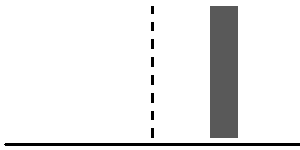
\includegraphics[width=0.06\textwidth]{../results/correlations/figures/posteriors/posterior_Real_lifted_mark.pdf}     } 
		&   \multirow{2}{*}{  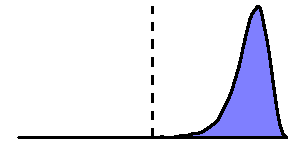
\includegraphics[width=0.06\textwidth]{../results/correlations/figures/posteriors/posterior_Efficiency_lifted_mark.pdf}     } 
		&   \multirow{2}{*}{  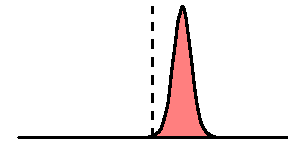
\includegraphics[width=0.06\textwidth]{../results/correlations/figures/posteriors/posterior_Predictability_lifted_mark.pdf}     } 
		&   \multirow{2}{*}{  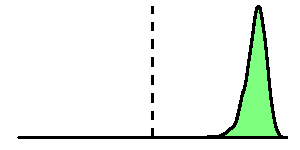
\includegraphics[width=0.06\textwidth]{../results/correlations/figures/posteriors/posterior_Parseability_lifted_mark.pdf}     } & \\
	&	\emph{that} & \emph{she has arrived}  &&&\\ \hline
	\multirow{2}{*}{	\raisebox{.5pt}{\textcircled{\raisebox{-.9pt} {7}}}}	&verb    &    PP         
		&   \multirow{2}{*}{  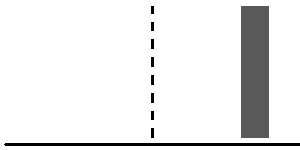
\includegraphics[width=0.06\textwidth]{../results/correlations/figures/posteriors/posterior_Real_obl.pdf}     } 
		&   \multirow{2}{*}{  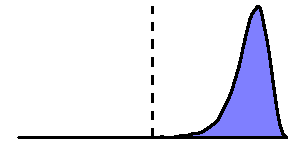
\includegraphics[width=0.06\textwidth]{../results/correlations/figures/posteriors/posterior_Efficiency_lifted_mark.pdf}     } 
		&   \multirow{2}{*}{  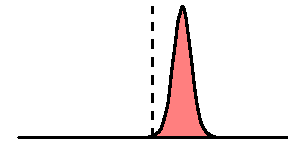
\includegraphics[width=0.06\textwidth]{../results/correlations/figures/posteriors/posterior_Predictability_lifted_mark.pdf}     } 
		&   \multirow{2}{*}{  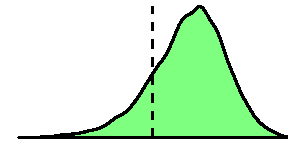
\includegraphics[width=0.06\textwidth]{../results/correlations/figures/posteriors/posterior_Parseability_obl.pdf}     } & \\
	&	\emph{went} & \emph{to school}  &&&\\ \hline
	\multirow{2}{*}{\raisebox{.5pt}{\textcircled{\raisebox{-.9pt} {8}}}}	&want    &    VP        
		&   \multirow{2}{*}{  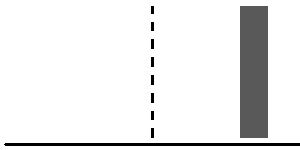
\includegraphics[width=0.06\textwidth]{../results/correlations/figures/posteriors/posterior_Real_xcomp.pdf}     } 
		&   \multirow{2}{*}{  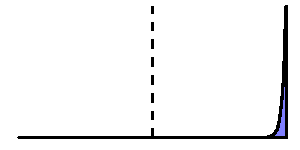
\includegraphics[width=0.06\textwidth]{../results/correlations/figures/posteriors/posterior_Efficiency_xcomp.pdf}     }
		&   \multirow{2}{*}{  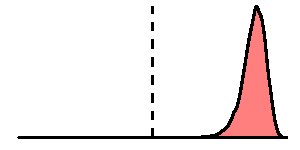
\includegraphics[width=0.06\textwidth]{../results/correlations/figures/posteriors/posterior_Predictability_xcomp.pdf}     }
		&   \multirow{2}{*}{  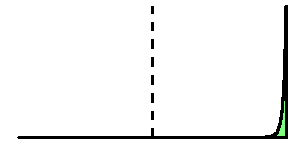
\includegraphics[width=0.06\textwidth]{../results/correlations/figures/posteriors/posterior_Parseability_xcomp.pdf}     } & \\
	& \emph{wants}   &  \emph{to leave}  &&&\\ \hline
 \hline
%comp. &
%\multirow{3}{*}{NP}&
%	AP &
%    \multicolumn{4}{l}{\footnotesize{Significance levels: $^*$: $p < 0.05$, : $p < 0.01$, : $p < 0.001$}}
\end{tabular}
	\end{center}
\caption{OPTION 3: Efficiency optimization accurately predicts the Greenbergian correlations. Each correlation is stated in terms of a pair of a `verb patterner' and an `object patterner', whose relative order correlate with that of verbs and objects.
For each correlation, we provide an English example, and show the distribution among the actual grammars of the 51 languages (left), and among grammars optimized for efficiency (right).
Blue bars count grammars conforming to the correlation, red bars count grammars violating it.
Efficiency optimization predicts all eight correlations to hold in the majority of grammars.
%Given the statistical nature of the correlations, not every language satisfies every one of them.
%Not all correlations are satisfied by every natu
}\label{table:corr-dryer}
\end{table*}



\begin{figure}
    \centering
    
    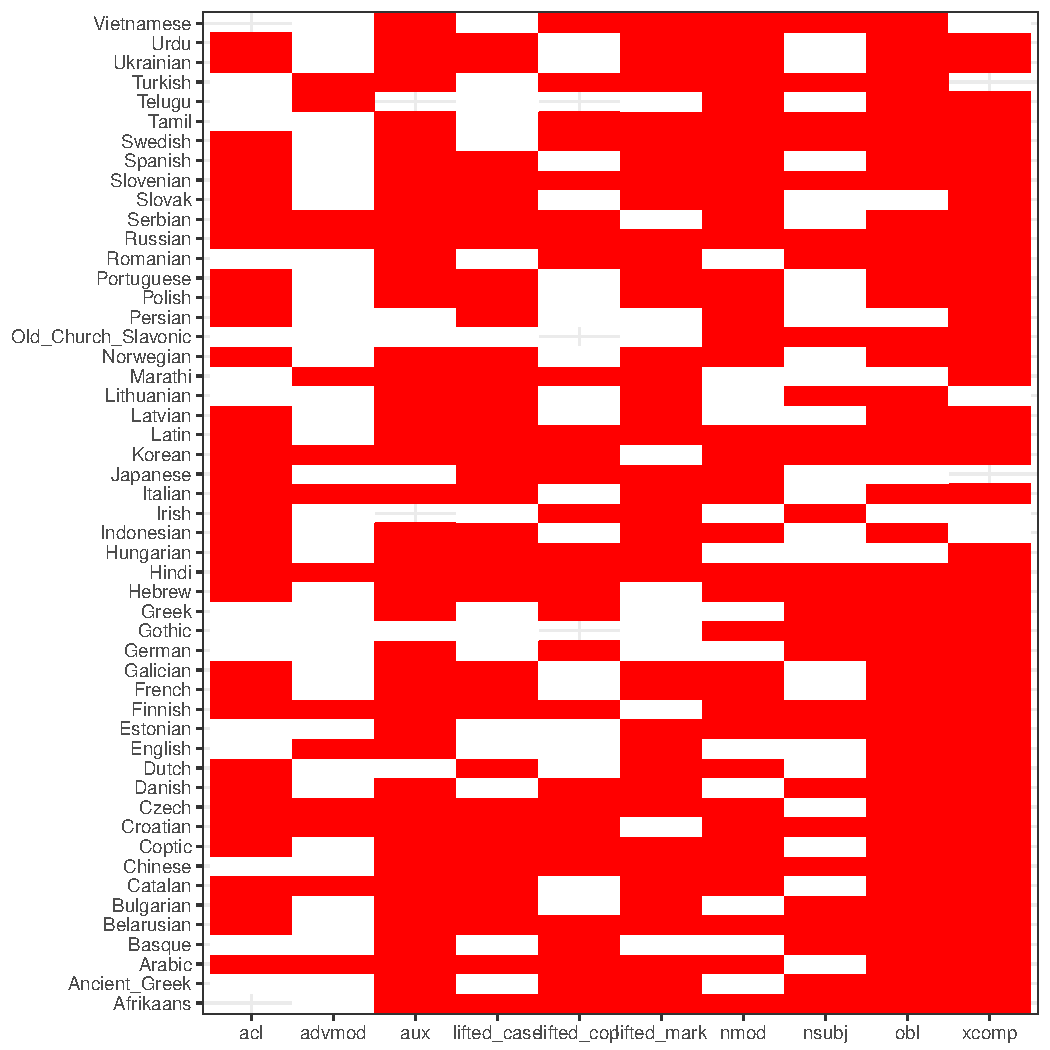
\includegraphics[scale=.25]{../results/correlations/figures/coverage-langmod-best.pdf}
    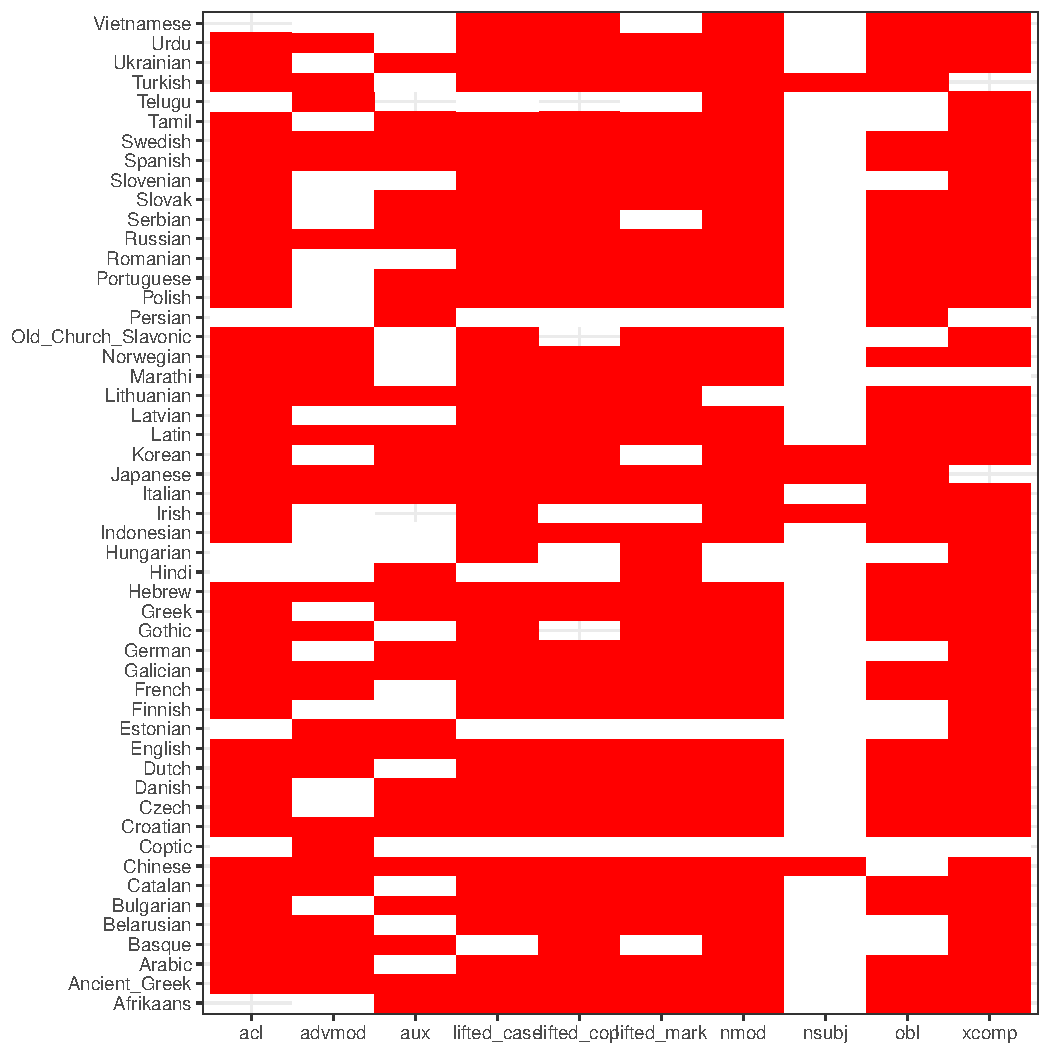
\includegraphics[scale=.25]{../results/correlations/figures/coverage-parse-best.pdf}
    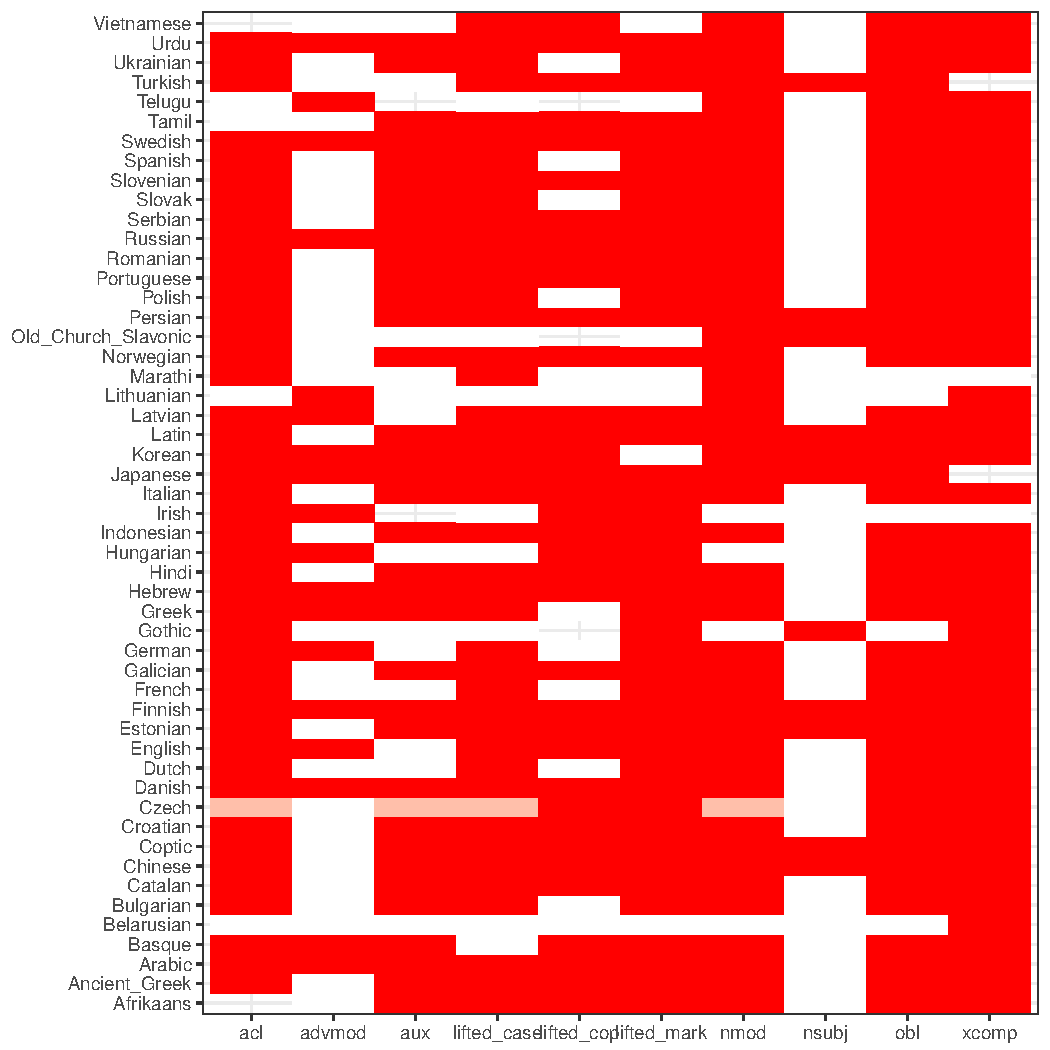
\includegraphics[scale=.25]{../results/correlations/figures/coverage-two-lambda09-best.pdf}
    
    
    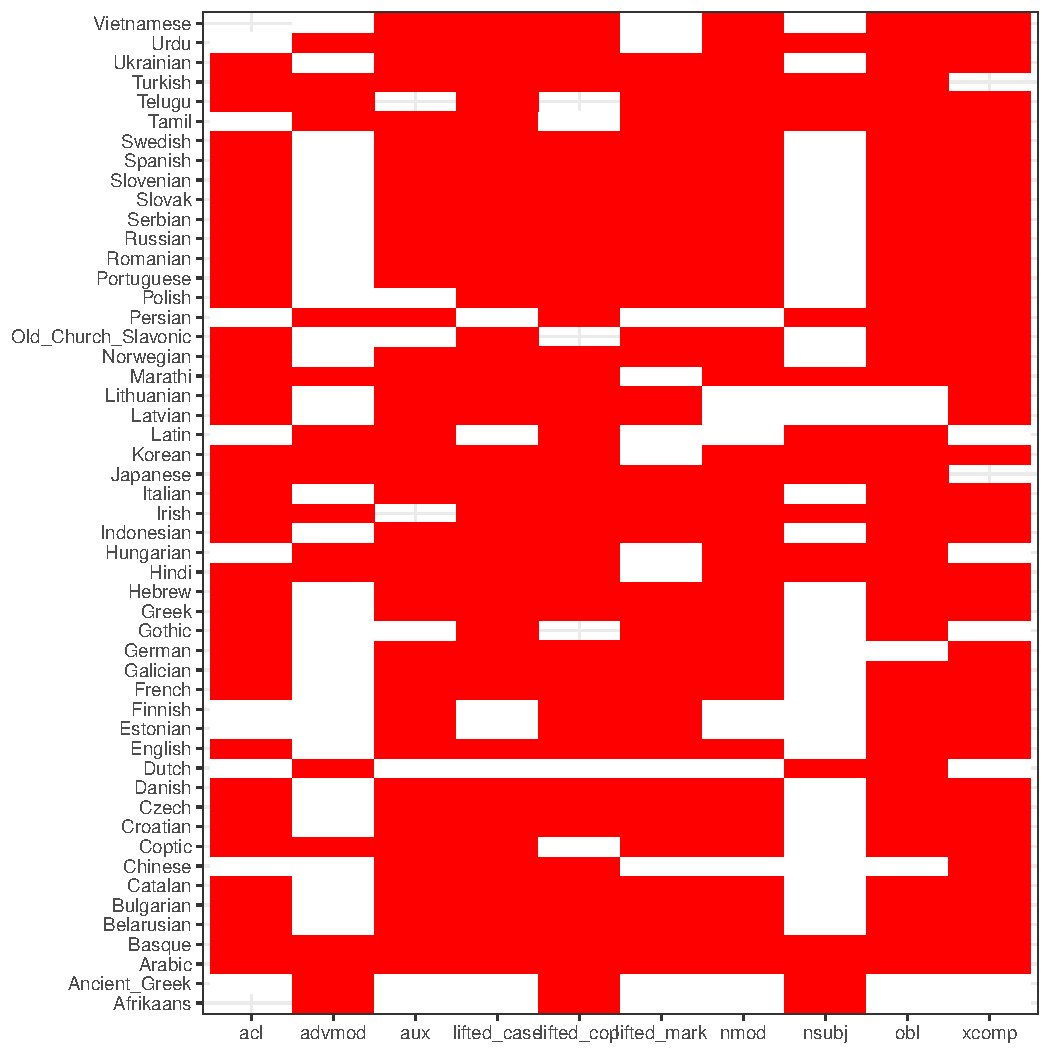
\includegraphics[scale=.25]{../results/correlations/figures/coverage-ground.pdf}
    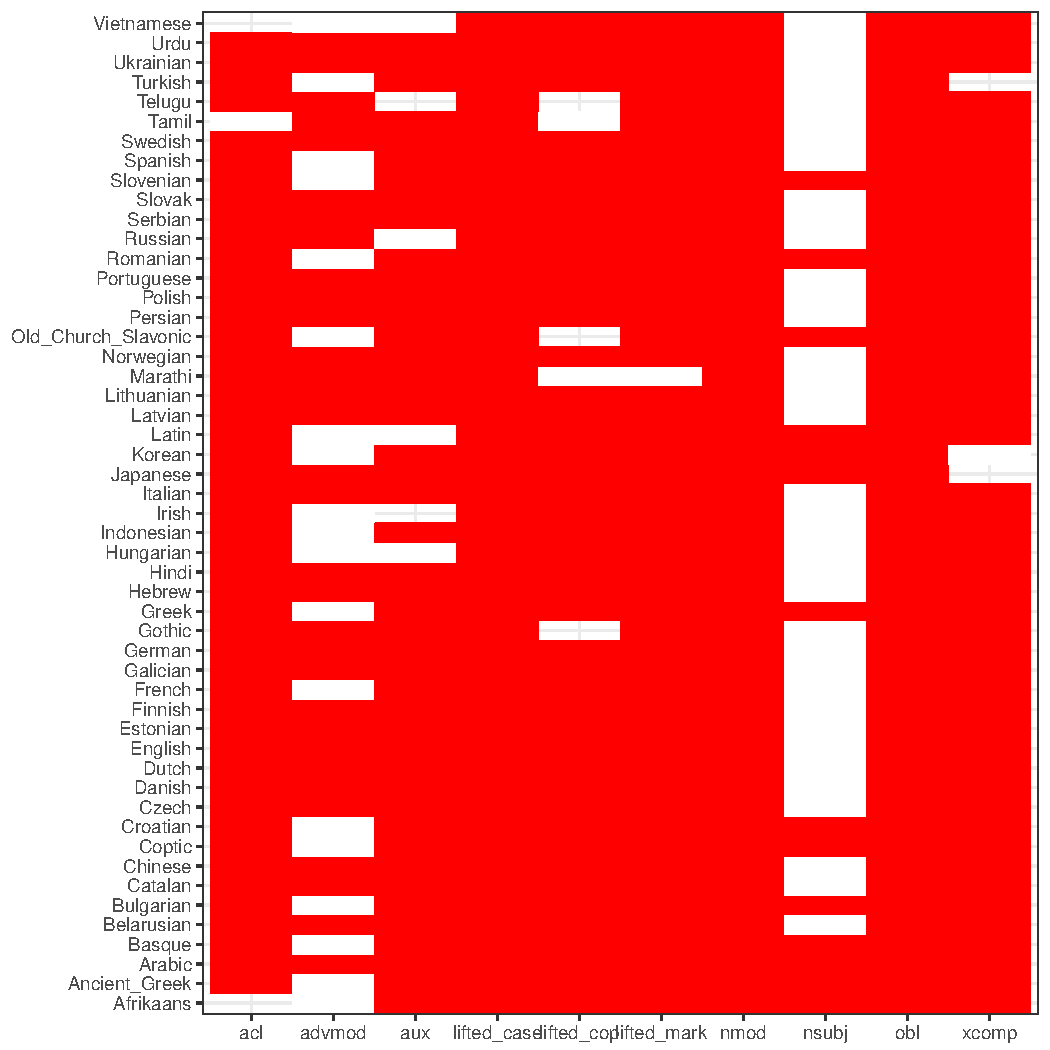
\includegraphics[scale=.25]{../results/correlations/figures/coverage-depl.pdf}
	\caption{Correlations satisfied by the best word order grammars for predictability, parseability, efficiency, by the UD languages, and by the best grammars for dependency length.}
    \label{fig:posterior-prevalence}
\end{figure}






\section{Relation to the Information Bottleneck}

Our efficiency objective (Equation~\ref{eq:efficiency}), to be maximized for word order grammars $L$, is restated below.
\begin{equation}
    \label{eq:efficiency-again}
    J_T(L) = I[L(T); T] - \lambda H[L(T)].
\end{equation}
This equation can be seen as a special case of the objective function proposed in \citet{tishby1999information} for general lossy compression, based on rate-distortion theory \citep{cover2006elements,harremoes2007information}. In that theory, the goal is to derive an encoding $\hat{X}=L(X)$ of some variable $X$ which preserves the information in $X$ relevant to some third variable $Y$, while minimizing irrelevant information. The three variables $Y$,$X$, and $\hat{X}$ are assumed to form a Markov chain $Y \rightarrow X \underrightarrow{L} \hat{X}$. Given those variables, the information bottleneck objective to be maximized is given in Eq.~\ref{eq:ib}.
\begin{equation}
    \label{eq:ib}
    J_{X,Y}(L) = I[\hat{X}; Y] - \lambda I[\hat{X}; X].
\end{equation}
In this equation, the joint distribution of $X$ and $Y$ is seen as fixed, and the conditional distribution $L=\hat{X}|X$ is optimized.

In our setting we consider a language $L$ expressing trees $T$ as utterances $U$: $T \underrightarrow{L} U$. To make our formulation more parallel to the information bottleneck, we assume the utterances $U$ are passed through a channel from producer to comprehender, and received as $\hat{U}=U$. We have the Markov chain $T \underrightarrow{L} U \rightarrow \hat{U}$, where we are assuming the conditional channel distribution $\hat{U}|U$ is fixed and the conditional distribution $L=U|T$ is to be optimized. Then our objective is parallel to Eq.~\ref{eq:ib}:
\begin{equation}
    \label{eq:efficiency-kinda-ib}
    J_T(L) = I[U;T] - \lambda I[U;\hat{U}]. % TODO should this be I[\hat{U};T]?
\end{equation}
Assuming the channel $U \rightarrow \hat{U}$ is noiseless, we have $U=\hat{U}$, and thus $I[U;\hat{U}]=I[U;U] = H[U]$. Then Eq.~\ref{eq:efficiency-kinda-ib} reduces to a form of Eq.~\ref{eq:efficiency-again}:
\begin{equation*}
    J_T(L) = I[U;T] - \lambda H[U].
\end{equation*}

Our efficiency objective is thus closely related to the information bottleneck; the difference is that we are optimizing the mapping from underlying meanings to representations (strings) assuming that these strings will be transmitted in a fixed noiseless channel.

\section{Possible values of $\lambda$}

In the efficiency objective~(\ref{eq:efficiency-again}), the value of $\lambda$ is constrained to be in $[0,1)$.
This means, surprisal must be weighted less strongly than parsability.

Greater values of $\lambda$ mathematically result in degenerate solutions.
To show this, note that the following inequality always holds:
\begin{equation}
I[L(T); T] \leq H[L(T)].
\end{equation}
Therefore, if $\lambda \geq 1$, the efficiency objective satisfies 
\begin{equation}
    J_T(L) = I[L(T); T] - \lambda H[L(T)] \leq 0.
\end{equation}
and it takes the maximally possible value zero if $L(T)$ maps all trees to a single utterance, in which case both $I[L(T); T]$ and $H[L(T)]$ are zero.
This is a degenerate language with only a single utterance, which is simultaneously used to convey all meanings.
While the design of our word order grammars precludes a collapse of all trees to a single utterance, this shows that an objective with $\lambda \geq 1$ cannot be a generally applicable objective for language efficiency.

In our experiments, we chose $\lambda = 0.9$ as a mathematically valid value that puts similar weight on both predictability and parsability.
We previously carried out language optimization for $\lambda = 1$, and obtained essentially identical predictions for word order correlations and relative optimality of language.

The computational cost of grammar optimization precluded repeating the experiment for many values of $\lambda$.
We note that each of the eight correlations is predicted by at least parseability or predictability, without any contradictory predictions (TODO check).

\section{Joint optimization of grammar, parser, and language model parameters}


\subsection{Differentiable Ordering Grammars}

In order to carry out optimization of grammars, we extend the space of grammars to include probabilistic relaxations of grammars, which describe probability distributions over different ways of ordering a syntactic structure into a sentence.
This makes efficiency a differentiable function of the grammar parameters, and enables optimization with stochastic gradient descent, as we describe in Section~\ref{sec:optim-eff}.

The parameters of such a differentiable word order grammar are as follows. 
For each dependency label type $\tau$, we have (1) a \key{Direction Parameter} $a_\tau \in [0,1]$, and (2) a \key{Distance Parameter} $b_\tau \in \mathbb{R}$. 
Each dependent is ordered on the left of its head with probability $a_\tau$ and to the right with probability $1-a_\tau$. 
Then for each set of co-dependents $\{s_1, \dots , s_n\}$ placed on one side of a head, their order outward from the head is determined by iteratively sampling from the distribution $\operatorname{softmax}(b_{\tau_1}, \dots, b_{\tau_n})$ (\cite{goodfellow2016deep}, p. 184) without replacement. 

If $a_\tau \in \{0, 1\}$, and the distances between values of $b_\tau$ (for different $\tau$) become very large, such a differentiable grammar becomes deterministic, assigning almost full probability to exactly one ordering for each syntactic structure.
In this case, the grammar can be converted into an equivalent grammar of the form described in Materials and Methods, by extracting a single parameter in $[-1, 1]$ for each relation $\tau$.

\subsection{Extracting Grammars from Datasets}
We extract grammars for the actual languages by fitting a differentiable ordering grammar maximizing the likelihood of the observed orderings.
To prevent overfitting, we regularize each $a_\tau$, $b_\tau$ with a simple Bayesian prior $logit(a_\tau) \sim \mathcal{N}(0,1)$, $b_\tau \sim \mathcal{N}(0,1)$.
We then extract the posterior means for each parameter $a_\tau, b_\tau$, and convert the resulting differentiable grammar into an ordinary ordering grammar.

\subsection{Optimizing Grammars for Efficiency}\label{sec:optim-eff}

\textbf{rewrite this}

For each of our objective functions, we seek parameters $\theta$ of a word order grammar $L_\theta$ that maximize the average utility of sentences in the language obtained by linearizing unordered trees $t \sim T$ according to $L_\theta$. The calculation of the predictability and parseability objectives also requires fitting language models parameterized by $\phi$ and parsers parameterized by $\psi$, respectively; and the calculation of the efficiency objective requires joint optimization of the word order grammar, language models, and parsers. The optimization problems come out to:
\begin{align}
\max_\theta &\E_{t \sim T}\E_{{\bf w} \sim L_\theta(t)} R_{DepL}(t; {\bf w}) \label{eq:maximize-depl}\\
\max_{\theta,\phi} &\E_{t \sim T}\E_{{\bf w} \sim L_\theta(t)} R_{Pred}^{\phi(\theta)}(t; {\bf w}) \label{eq:maximize-pred}\\
\max_{\theta,\psi} &\E_{t \sim T}\E_{{\bf w} \sim L_\theta(t)} R_{Pars}^{\psi(\theta)}(t; {\bf w}) \label{Eq:maximize-pars} \\
\max_{\theta,\phi,\psi} &\E_{t \sim T}\E_{{\bf w} \sim L_\theta(t)} R_{Efficiency}^{\psi(\theta), \phi(\theta)}(t; {\bf w}). \label{eq:maximize-efficiency} 
\end{align}
Note that the original word orders from the treebank never enter this objective---in particular, they do not influence the language model and the parser, which are entirely determined by $\theta$.

The case of dependency length in Eq.~\ref{maximize-depl} is the simplest, requiring only coordinate descent on the parameters $a_\tau, b_\tau \in \theta$. A similar optimization problem was solved by hill-climbing in \citet{gildea2007optimizing} and \citet{gildea2015human}.
We optimize this objective by stochastic gradient descent with a batch size of one unordered dependency tree.

The case of predictability, parseability, and efficiency are more challenging, as we need to simultaneously look for an ordering model optimized for the loss of a language model and/or a parser, and for a language model and/or parser that are optimized for that given ordering model.
We solve Eqs.~\ref{eq:maximize-pred}--\ref{eq:maximize-efficiency} by performing stochastic gradient descent over all sets of parameters $\theta, \phi$, and/or $\psi$ simultaneously.
Below we discuss the process only for the predictability objective (Eq.~\ref{eq:maximize-pred}); the other objectives are optimized analogously.
In each step, we sample a dependency tree $t$ from the treebank, then sample an ordering from the current setting of $\theta$ to obtain a linearized sentence ${\bf w} \sim P_{L_\theta}(\cdot|t)$.
Then we %update $\thetal$ with ordinary gradient descent, and $\thetad$ with the REINFORCE estimator~\ref{williams-simple-1992}.
do a gradient descent step using the estimator %(analogous for $R_{Pars}$ instead of $R_{Pred}$)
\begin{equation}\label{eq:estimator}
{ \partial_\theta \left(\log P_{L_\theta}({\bf w}|t)\right) \cdot R^\phi_{Pred} (t; {\bf w}) \choose  \partial_\phi R_{Pred}^\phi(t; {\bf w})}
%{- \partial_\thetad \left(\log P_\thetad({\bf w})\right) \cdot R_{Pred}(\bf{w}, \thetal) \choose  - \partial_\thetal \sum_{i=1}^{\#{\bf w}} \log P_\thetal(w_{i+1}|w_{1\dots i})}
\end{equation}
%$${- \partial_\thetad \left(\log P_\thetad({\bf w})\right) \cdot \sum_{i=1}^{\#{\bf w}} \log P_\thetal(w_{i+1}|w_{1\dots i}) \choose  - \partial_\thetal \sum_{i=1}^{\#{\bf w}} \log P_\thetal(w_{i+1}|w_{1\dots i})}$$
for the gradient
$${ \partial_\theta \choose \partial_\phi} \E_{{\bf w'} \sim L_\theta(t)} R_{Pred}^\phi(t; {\bf w'}).$$
This unbiased estimator is the ordinary gradient estimator for $\phi$, and the REINFORCE estimator for $\theta$ \citep{williams1992simple}.

In addition, we estimated maximum-likelihood ordering grammars on the original ordered dependency trees with SGD. For nonprojective trees, we ignore discontinuities.
%and $\ell_2$ regularization.

A different commonly considered information-theoretic objective function for word order is Uniform Information Density~\citep{jaeger2010redundancy}, formalized as minimizing a superlinear function of per-word surprisal~\citep{levy:2018cogsci}.
Note that optimizing grammars for this objective faces additional challenges, as the optimization problem cannot be rewritten as joint optimization in the form (\ref{eq:maximize-pred}).
We thus do not evaluate this objective function here.




%We extract grammars for the actual languages using a Bayesian data analysis method.
%We specify a simple Bayesian prior over differentiable ordering grammars:
%$$logit(a_\tau) \sim \mathcal{N}(0,1),\ \ \ \ b_\tau \sim \mathcal{N}(0,1)$$
%for each $\tau$.
%Recall that, given a syntactic structure, a differentiable ordering grammar assigns a probability distribution over possible orderings.
%We extract 


\section{Neural Network Architectures}

In this section, we describe the details of the neural network architectures.
All choices described in this section were fixed before evaluating word order properties and the efficiency of real language.

%\paragraph{Locality}
%In Equation~\ref{eq:depl}, we assume that $head(w_i) = i$ iff $w_i$ is the root of the sentence, so that the root does not contribute to dependency length.

\paragraph{Estimating Predictability}
We choose a standard LSTM \citep{hochreiter1997long} language model with vocabulary size restricted to the most frequent 50,000 words in the treebanks for a given language.
Given the small size of the corpora, this limit is only attained only for few languages.
In each time step, the input is a concatenation of embeddings for the word, for language-specific POS tags, and for universal POS tags.
The model predicts both the next word and its POS tags in each step.
Using POS tags is intended to prevent overfitting on small corpora.
These decisions were made before evaluating word order properties.

\paragraph{Estimating Parseability}
We use a biaffine attention parser architecture \citep{kiperwasser2016simple,zhang2017dependency,dozat2017stanford}. This architecture is remarkably simple: the words of a sentence are encoded into context-sensitive embeddings using bidirectional LSTMs, then a classifier is trained to predict the head for each work. The classifier works by calculating a score for every pair of word embeddings $(w_i, w_j)$, indicating the likelihood that the $j$th word is the head of the $i$th word. This is a highly generic architecture for recovering graph structures from strings, and is a simplification of graph-based parsers which reduce the parsing problem to a minimal spanning tree problem \citep{mcdonald2005nonprojective}.

To reduce overfitting on small corpora, we choose a delexicalized setup, parsing only from POS tags. Preliminary experiments showed that a parser incorporating word forms overfitted long before the ordering model had converged; parsing from POS tags prevents early overfitting.
This decision was made before evaluating word order properties.

\paragraph{Hyperparameters}

\textbf{TODO study 1 only has 1 set of parameters}

Neural network models have hyperparameters such as the number of hidden units, and the learning rate. 
For predictability and parseability optimization, we first selected hyperparameters on the respective objectives for selected languages on the provided development partitions.
Then, for each language and each objective function, we created eight random combinations of these selected hyperparameter values, and selected the setting that yielded the best value of the respective objective function (predictability or parseability) on the language. We then used this setting for creating optimized word order grammars. 

\textbf{TODO random seeds for efficiency}

All word and POS embeddings are randomly initialized with uniform values from $[-0.01, 0.01]$.
We do not use pretrained embeddings \citep{peters2018deep}: While these could improve performance of language models and parsers, they would introduce confounds from the languages' actual word orders as found in the unlabeled data.


%\begin{table}[]
%    \centering
%    \begin{tabular}{c|cccc}
%    Entropy penalty     &  0.0001, 0.001 \\
%    Learning Rate (Word order grammar)     & 5e-6, 1e-5, 2e-5, 5e-5 \\
%    Momentum (Word order grammar) & 0.8, 0,9 \\
%    Dropout (Language model) & 0.0, 0.3, 0.5 \\
%    
%    \end{tabular}
%    \caption{Hyperparameters}
%    \label{tab:my_label}
%\end{table}

\paragraph{Optimization details}

We employ two common variance reduction methods to improve the estimator~(\ref{eq:estimator}), while keeping it unbiased.
%For dependency length and 
For predictability, note that the loss incurred for a specific word only depends on ordering decisions made up to that word (and its head, in the case of dependency length). We represent the process of linearizing a tree as a dynamic stochastic computation graph, and use these independence properties to apply the method described in \citet{schulman2015gradient} to obtain a version of~(\ref{eq:estimator}) with lower variance.
Second, we use a word-dependent moving average of recent per-word losses as control variate \cite{williams1992simple}.
These two methods reduce the variance of the estimator and thereby increase the speed of optimization and reduce training time, without biasing the results.
For numerical stability, we represent $a_\tau \in [0,1]$ via its logit $\in \mathbb{R}$.
Furthermore, to encourage exploration of the parameter space, we add an entropy regularization term \citep{xu2015show} for each Direction Parameter $a_\tau$, which penalizes $a_\tau$ values near $0$ or $1$. The weight of the entropy regularization was chosen together with the other hyperparameters.
%, adding the negative entropy of the $Bernoulli(a_\tau)$ to the loss $R$. %, weighted with $\alpha$.


These techniques for improving (\ref{eq:estimator}) are well-known in the machine learning literature, and we fixed these before evaluating optimized grammars for word order properties.

We update word order grammar parameters $\theta$ using Stochastic Gradient Descent with momentum.
For the language model parameters $\phi$, we use plain SGD. 
For the parser parameters $\psi$, we use Adam \citep{kingma2014adam}, following \citet{dozat2017stanford}.
The learning rates and other optimization hyperparameters were determined together with the other hyperparameters.

For each language and objective function, we apply Early Stopping~\citep{prechelt1998early} as follows. We compute a Monte-Carlo estimate of the objective on the UD development set in intervals of 50,000 training steps, and stop optimization once the value of the objective deteriorates compared to the last previous estimate. This technique, well known in the machine learning literature, helps prevent overfitting to the specific corpora used.

The choice of optimization methods and the stopping criterion were fixed before we investigated word order correlations.

Recall that, for each language, we created 8 optimized languages for each optimization criterion.
We enforced balanced distribution of object-verb and verb-object ordering among optimized languages by fixing $a_\tau$ for the \textit{obj} dependency to be 0.0 in four of these languages, and 1.0 in the other four.
This maximizes statistical precision in detecting and quantifying correlations between the \textit{obj} relation and other relations.



 % TODO we could use some language at the top of this section on the general guiding principles for all these decisions. Were these implementation decisions made before or after looking at the word order universals results? If they were made before, we should highlight that.


\section{Robustness to different language models and parsers}

Here we take up the question of the extent to which our results are dependent on the particular parser and language model used in the optimization process. We want to know: when we optimize a word order grammar for efficiency, have we produced a language which is highly efficient \emph{in general}, or one which is highly efficient \emph{for a specific parser}? We wish to argue that natural language syntax is optimized for efficiency in general, meaning that syntactic trees are highly recoverable from word orders in principle. If it turns out that our optimized languages are only optimal for a certain parser from the NLP literature, then we run the risk of circularity: it may be that the reason this parser was successful in the NLP literature was because it implicitly encoded word order universals in its inductive biases, and thus it would be no surprise that languages which are optimized for parseability also show those universals.

In this connection, we note that the parser and language model architectures we use are highly generic, and do not encode any obvious bias toward natural-language-like word orders. The LSTM language model is a generic model of sequence data which is also been used to model financial time series \citep{sirignano2018universal} and purely theoretical chaotic dynamical systems \citep{ogunmolu2016nonlinear}; the neural graph-based parser is simply solving a minimal spanning tree problem \citep{mcdonald2005nonprojective}. Nevertheless, it may be the case that a bias toward word order universals is somehow encoded implicitly in the hyperparameters and architectures of these models.

Here we address this question by demonstrating that our languages optimized for prediction and parseability are also optimal under a range of different language models and parsers. These results show that our optimization process creates language in which strings are generally predictable and informative about trees, without dependence on a particular prediction and parsing algorithms.

\subsection{CKY Parsers}


We constructed simple Probabilistic Context-Free Grammars (PCFGs) from corpora and word order grammars, using a simplified version of the models of Collins 1997 (Model 1).
In our PCFGs, each head independently generates a set of left and right dependents.
We formulate this as a PCFG where each rule has the form:
\begin{center}
	POS$_H$ $\rightarrow$ POS$_H$ POS$_D$
\end{center}
for head-initial structures, and
\begin{center}
	POS$_H$ $\rightarrow$ POS$_D$ POS$_H$
\end{center}
for head-final structures, where each symbol is a POS tag.
Thus, POS tags act both as terminals and as nonterminals.

We estimated probabilities by taking counts in the training partition, and performing Laplace smoothing with a pseudocount $\alpha=1$ for each possible rule of this form.
For such a PCFG, exact parsing is possible using Dynamic Programming, and specifically the CKY algorithm.

This parsing strategy is very different from the neural graph-based parser:
While the graph-based parser solves a minimum spanning tree problem, the CKY algorithm uses dynamic programming to compute the exact probabilities of trees given a sentence, as specified by the generative model encoded in the PCFG.
Second, while the graph-based neural parser uses machine learning to induce syntactic knowledge from data, the CKY parser performs exact probabilistic inference.
%In this sense, the CKY algorithm does not have any architectural biases in itself.
%On the other hand, the PCFG makes severely simplifying independence assumptions, compared to the universal approximation capabilities of neural network-based systems.

We used the CKY algorithm to compute the parsing loss $H[T|L_\theta(T)]$ on the validation partition of the English UD corpora, for random and optimized ordering grammars.
Results (Figure~\ref{fig:cky-parser}) show that optimized grammars are more parseable for exact parsing of a simple PCFG.
% TODO get UAS for compatibility with other parts of SI
%We then compared parsability of random and optimized word order grammars on English data.


\begin{figure}
    \centering
    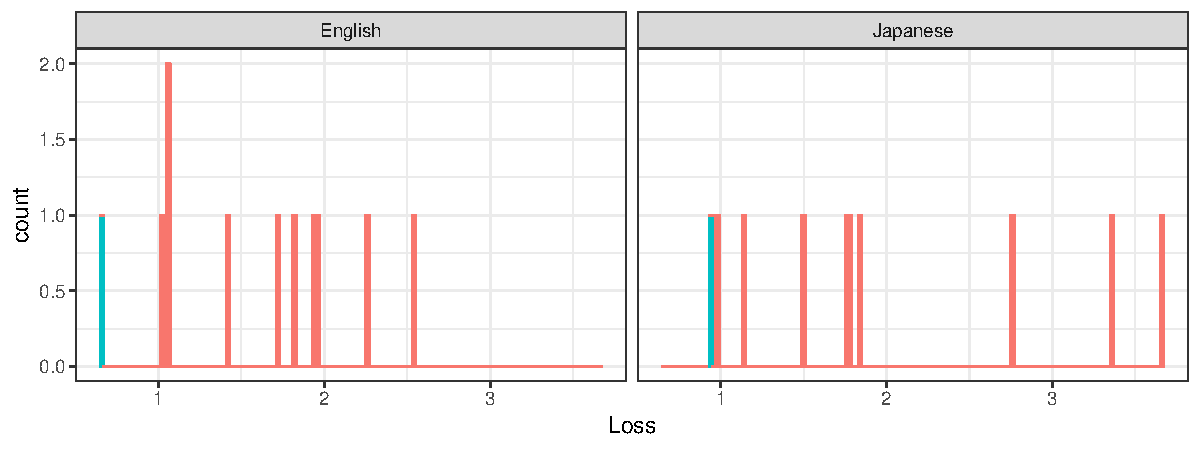
\includegraphics[scale=.7]{../results/cky/cky-parse.pdf} 
	\caption{Parsability loss $H[T|L_\theta(T)]$ (lower is better) computed by a simple CKY parser, for random word order grammars (red) and word order grammars optimized for efficiency (blue).}
    \label{fig:cky-parser}
\end{figure}



\subsection{Distorted graph-based parsers}

Many of the word order biases explained by parseability in Table~\ref{tab:result-dryer} are also explained by dependency length minimization. Therefore, we address here the idea that the graph-based parser might have a built-in bias toward parses involving short dependencies, which we call a \key{locality bias}.

A simple way to eliminate or alter a locality bias for any parser would be to change the order in which the parser sees words. Suppose that a parser $P$ has a bias toward positing a dependency between a word and the immediate previous word. 

\paragraph{Even--odd order.} A sequence of $n$ words originally ordered as $w_1 w_2 w_3 w_4 \cdots w_n$ is reordered by separating the even and odd indices: $w_2 w_4 w_6 \cdots w_{n-1} w_1 w_3 w_5 \cdots w_n$ (assuming $n$ odd). Therefore all words that are adjacent in the original order will be separated by a distance of $\approx n/2$ in the distorted order, while all words of distance 2 in the original order will become adjacent.

\paragraph{Interleaving order.} In interleaving ordering, a sequence originally ordered as $w_1 w_2 w_3 \cdots w_n$ is split in half at the middle (index $m=\ceiling{n/2}$), and the two resulting sequences are interleaved, yielding $w_1 w_m w_2 w_{m+1} w_3 w_{m+3} \cdots w_n$. Thus all words that were originally adjacent will have distance 2 in the distorted order, with the intervening word coming from a very distant part of the sentence.

\paragraph{Inwards order.} A sequence originally ordered as $w_1 w_2 w_3 \cdots w_{n-1} w_n$ is ordered from the edges of the string inwards, as $w_1 w_n w_2 w_{n-1} \cdots w_{\ceiling{n/2}}$. This corresponds to folding the string in on itself once, or equivalently, splitting the sequence in half at the middle, then interleaving the two resulting sequences after reversing the second one. The result is that the most non-local possible dependencies in the original order become the most local dependencies in the distorted order.

\paragraph{Sorted order.} A sequence is reordered by sorting by POS tags, and randomizing the order within each block of identical POS tags.
To each word, we then add a symbol encoding the original position in the sequence.
For instance
\begin{center}
PRON VERB PRON
\end{center}
may be reordered as
\begin{center}
PRON 1 PRON 3 VERB 2
\end{center}
or
\begin{center}
PRON 3 PRON 1 VERB 2
\end{center}
The numbers are provided to the parser as atomic symbols from a vocabulary ranging from 1 to 200; numbers greater than 200 (which may occur in extremely long sentences) are replaced by an out-of-range token.


\paragraph{Experiments}
Using English and Japanese data, we trained parsers for the ten random word order grammars and for the best grammar optimized for efficiency, with the input presented in each of the distorted orderings.
Resulting parsing accuracy scores are shown in Figure~\ref{fig:distorted-parser}.
In all settings, the language optimized for efficiency achieved higher parsing accuracy than random ordering grammars, showing that the parser's preference for optimized languages cannot be attributed to a locality bias.
%Note that absolute values of parsing accuracy vary between the orderings, being higher for the actual orderings than for distorted orderings, in which trees become nonprojective.

\begin{figure}
    \centering
    English
    
    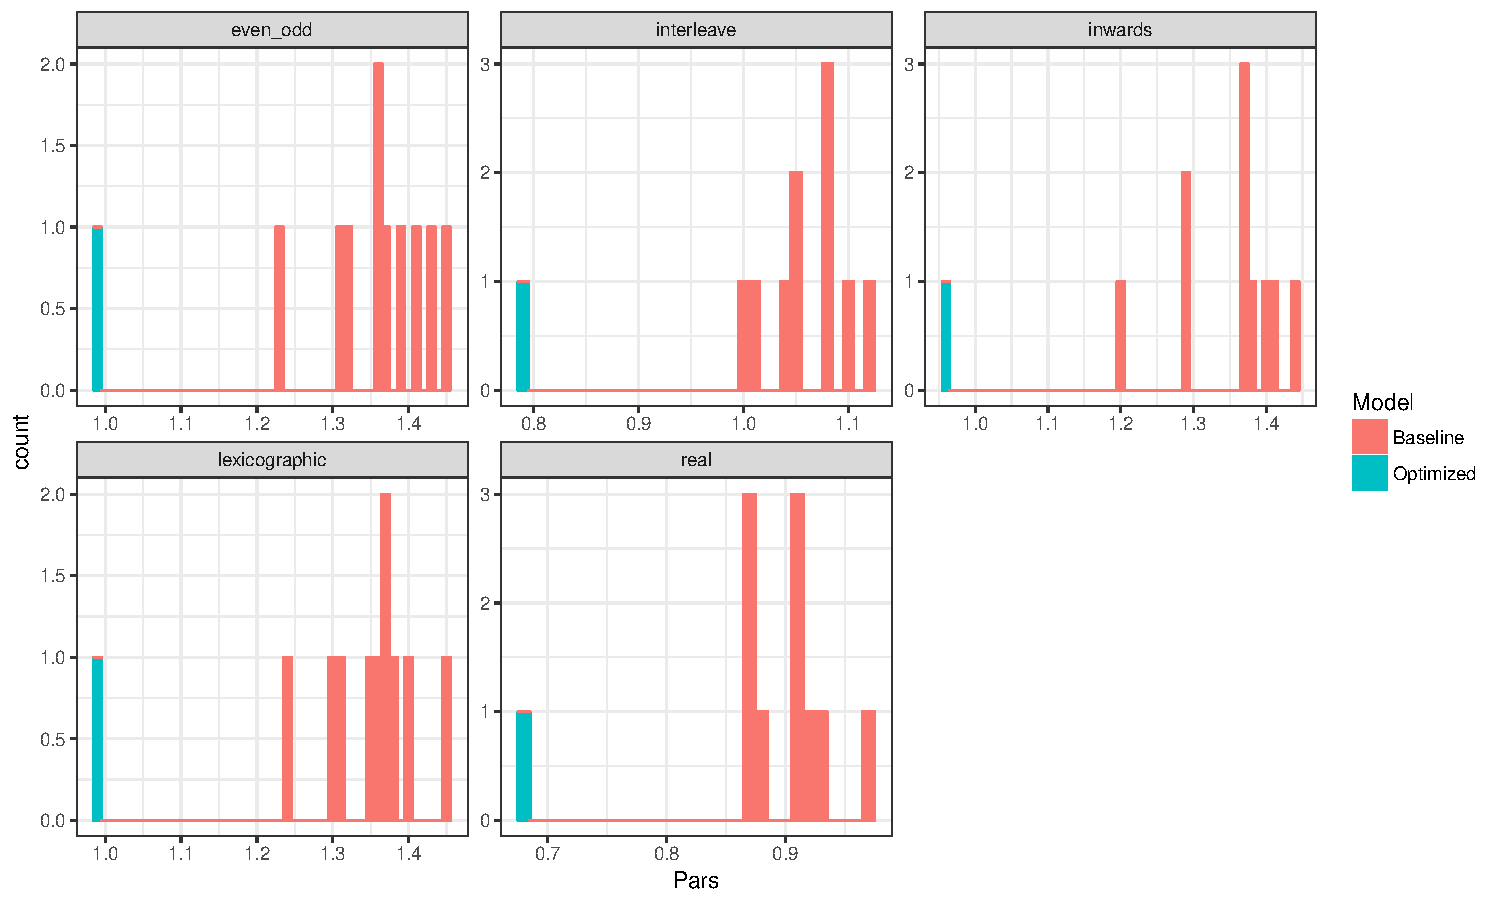
\includegraphics[scale=.5]{../results/permuted/adversarial-parse-loss-english.pdf}
    
    Japanese
    
    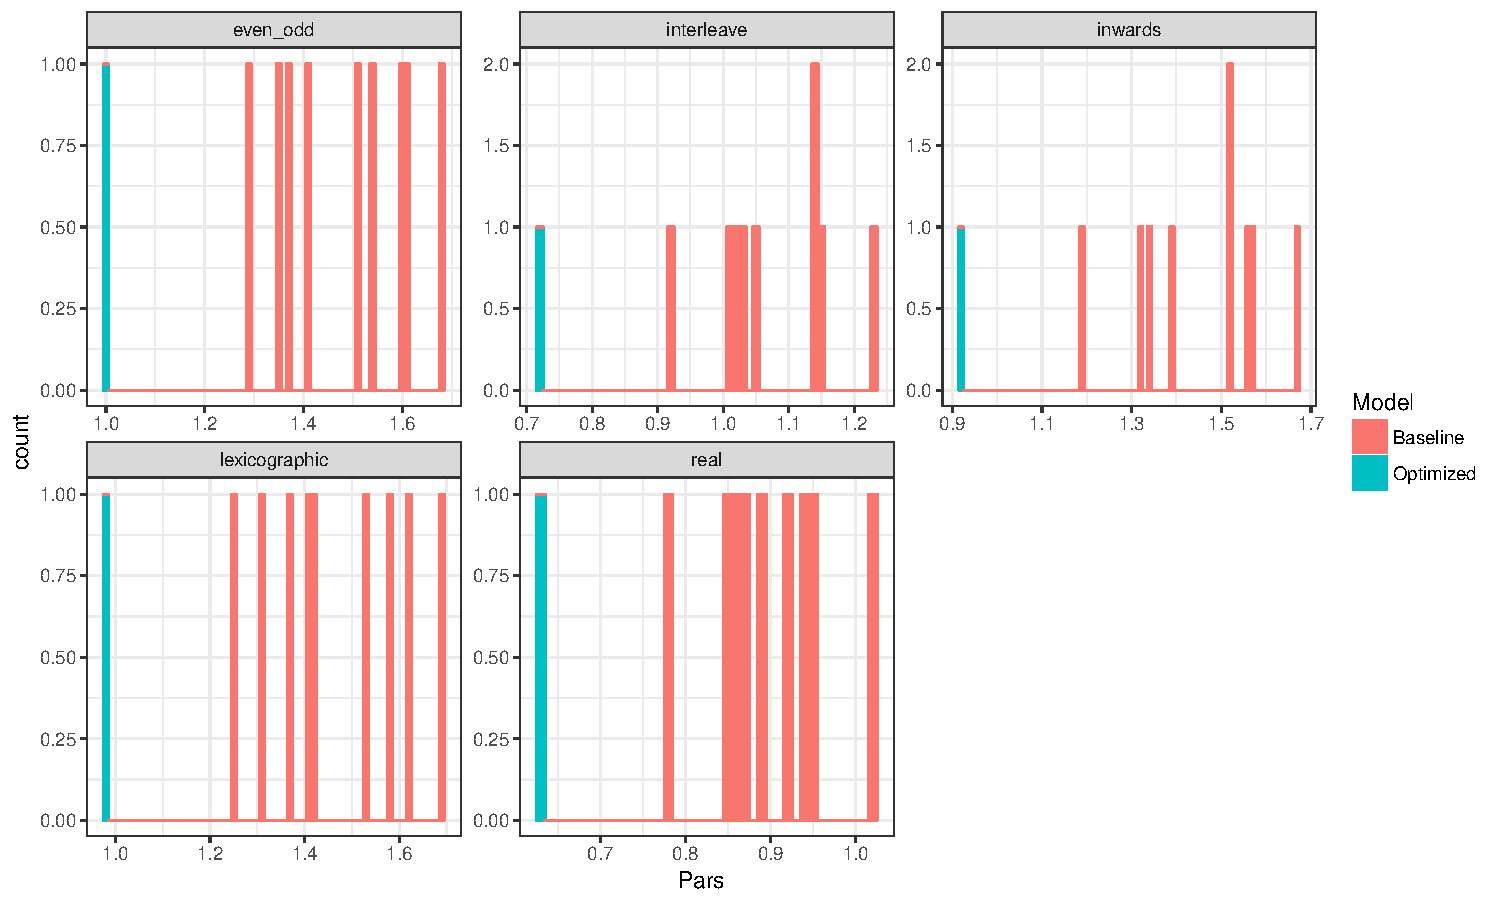
\includegraphics[scale=.5]{../results/permuted/adversarial-parse-loss-japanese.pdf}
	\caption{Parseability of baseline grammars and grammars optimized for efficiency, in English (top) and Japanese (bottom), measured by parsing loss $H[T|L_\theta(T)]$ (lower is better), for the four distorted orderings, and the actual orderings (`real').}
    \label{fig:distorted-parser}
\end{figure}


\subsection{n-gram language models}


We constructed a Bigram model with Kneser-Ney smoothing.
A bigram model predicts each word taking only the previous word into account.
This contrasts with LSTMs, which take the entire context into consideration.
Thus, bigram models and LSTMs stand on opposing ends of a spectrum of language models taking more and more aspects of the context into account.

We estimated language models on the training partitions, and used the validation partitions to estimate surprisal.
We conducted this for the ten random and the best optimized ordering grammars on English and Japanese data.
Results (Figure~\ref{fig:bigrams}) show that languages optimized for efficiency are optimal for a bigram language model.

\begin{figure}
    \centering
    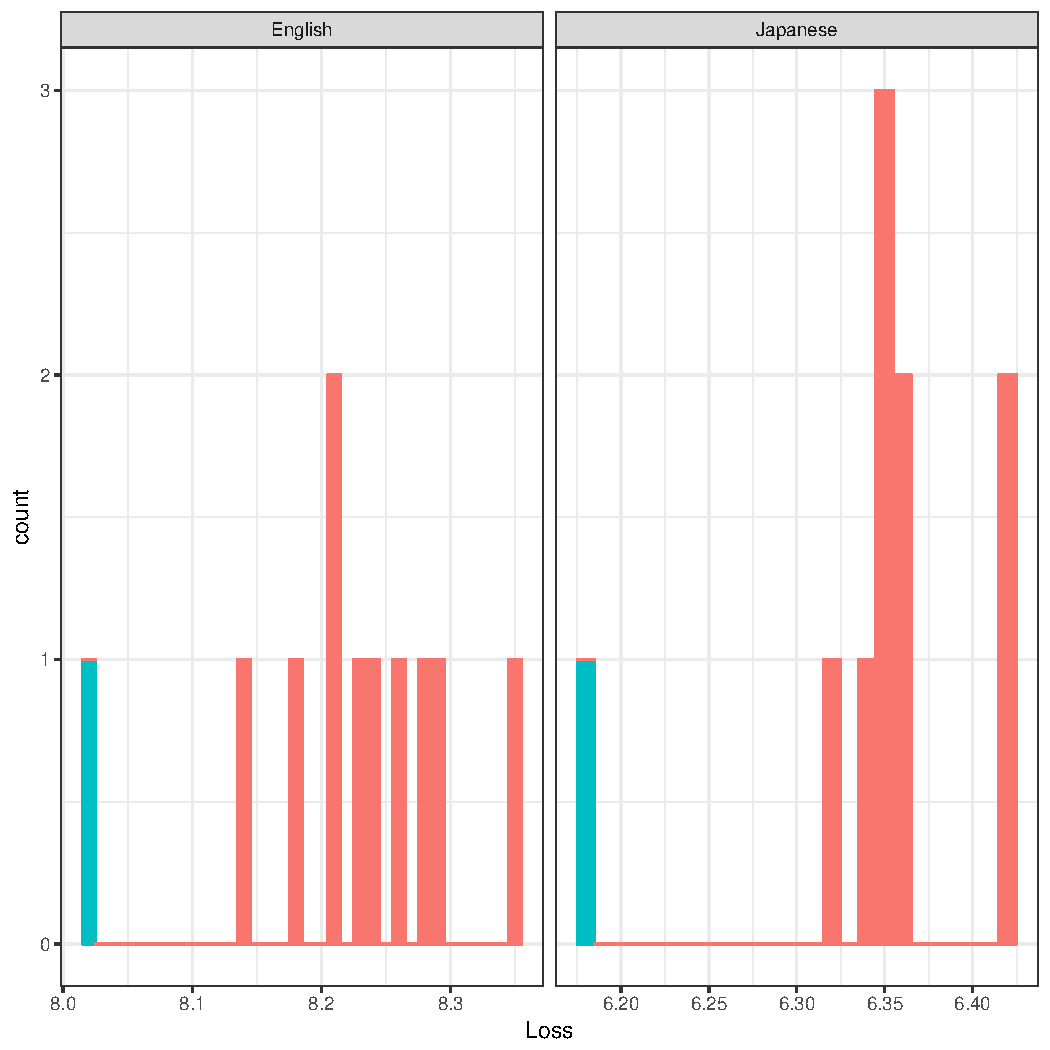
\includegraphics[scale=.4]{../results/bigrams/bigrams.pdf} 
	\caption{Surprisal (lower is better) computed from Bigram model, on English and Japanese data ordered according to random ordering grammars (red) and ordering grammars optimized for efficiency (blue).}
    \label{fig:bigrams}
\end{figure}




\subsection{Discussion}

It is always a logical possibility in studies such as this one that the results are dependent on the particular probabilistic models used. 

\section{Effects of data sparsity}

Here, we investigate whether the difference between real and baseline grammars is affected by the size of available datasets.
If the difference between random and real grammars is due to data sparsity, we expect that it decreases as the amount of training data is increased.
If, on the other hand, there is an inherent difference in efficiency between random and real grammars, we expect that the difference persists as training data is increased.

We considered Czech, the UD language with the largest amount of available treebank data (approx. 2.2 Million words), up to $\approx$ 300 times more data than is available for some other UD languages.
We cosidered both a random ordering grammar, and the best ordering grammar optimized for parseabaility.
For both of these ordering grammars, we trained the parser on successively larger portions of the training data (0.1 \%, 1 \%, 5\%, 10\%, 20 \%, ..., 90 \%, 100 \%) and recorded parsing accuracy.
Furthermore, for the random grammar, we varied the number of neurons in the BiLSTM (200, 400, 800) to test whether results depend on the capacity of the network.

\textbf{do same for language model, and for the other random grammars}

The resulting curves are shown in Figure~\ref{fig:learning-czech}.
A gap in parsing accuracy of about 0.07-0.1 appears already at 0.01 \% of the training data (2000 words), and persists for larger amounts of training data.

\begin{figure}
    \centering
    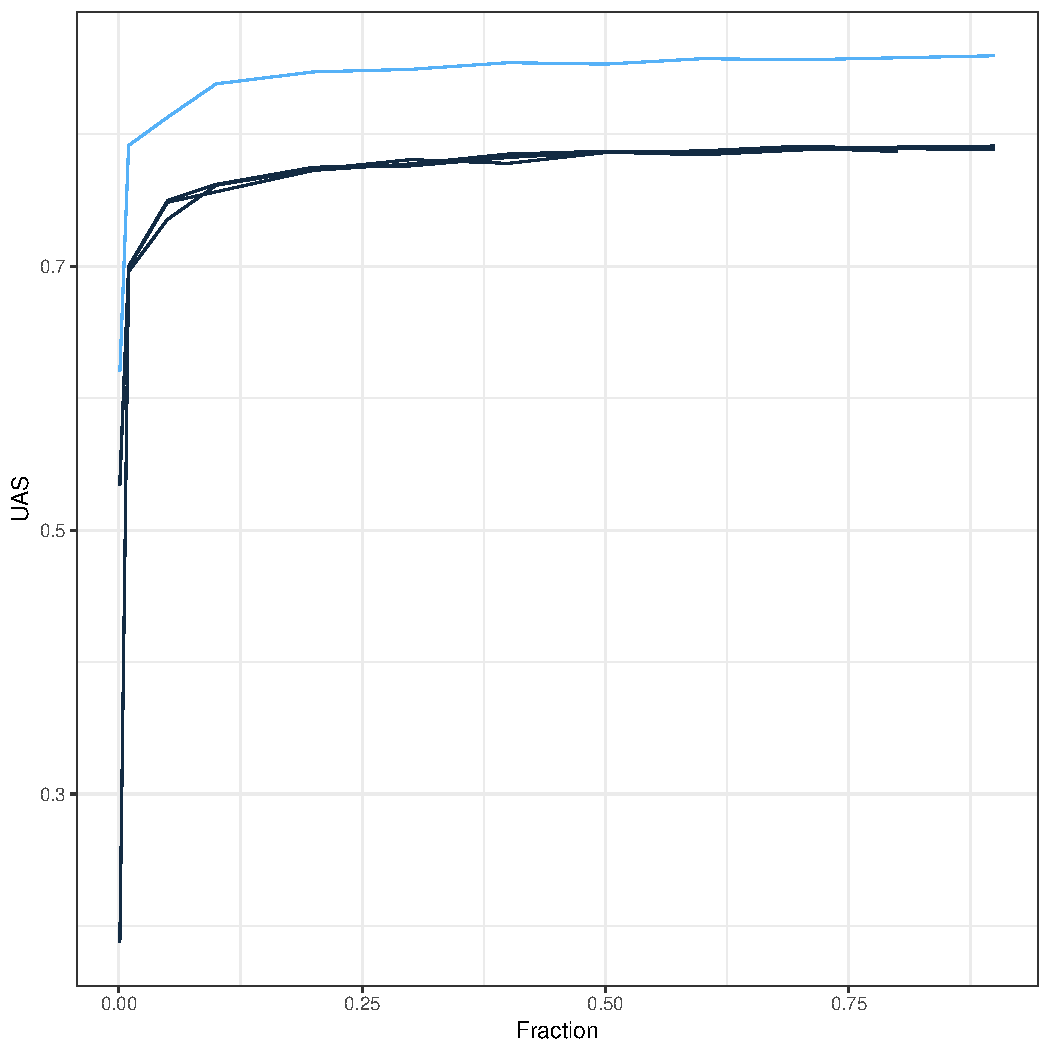
\includegraphics[scale=.4]{figures/learning-parser-czech.pdf} 
        \caption{Parsing accuracy (measured in UAS) for optimized (light blue) and random (black) ordering grammar on Czech data, as a function of the fraction of total training data provided.}
    \label{fig:learning-czech}
\end{figure}





\section{Study 2, Correlation between Universals and Efficiency}


\begin{figure}
    \centering
    
    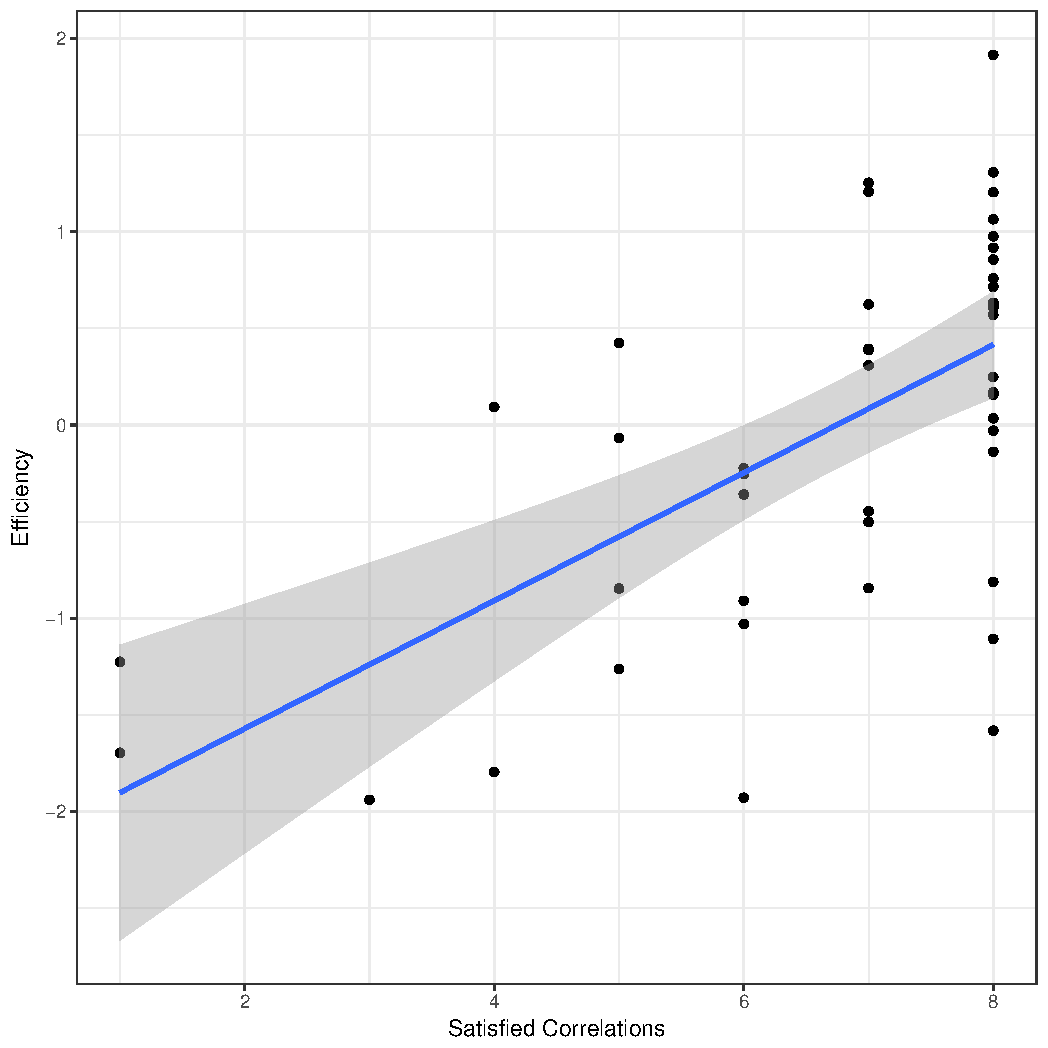
\includegraphics[scale=.25]{../results/correlations/correlations-by-grammar/ground-corrs-efficiency.pdf}
    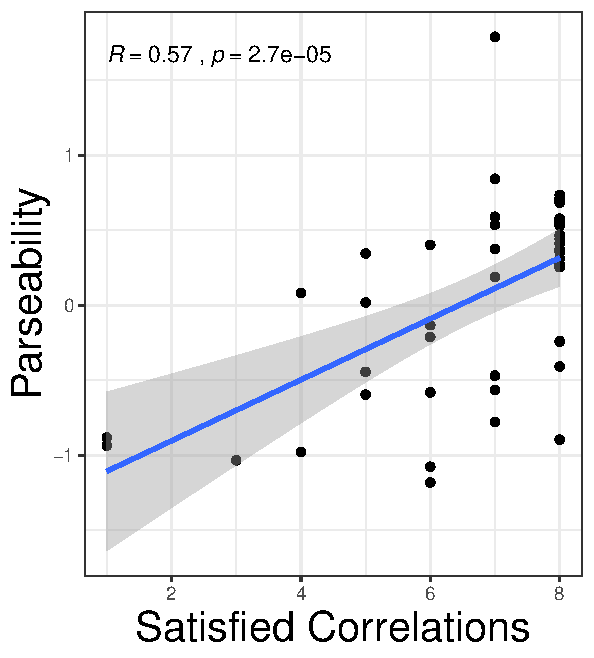
\includegraphics[scale=.25]{../results/correlations/correlations-by-grammar/ground-corrs-parseability.pdf}
    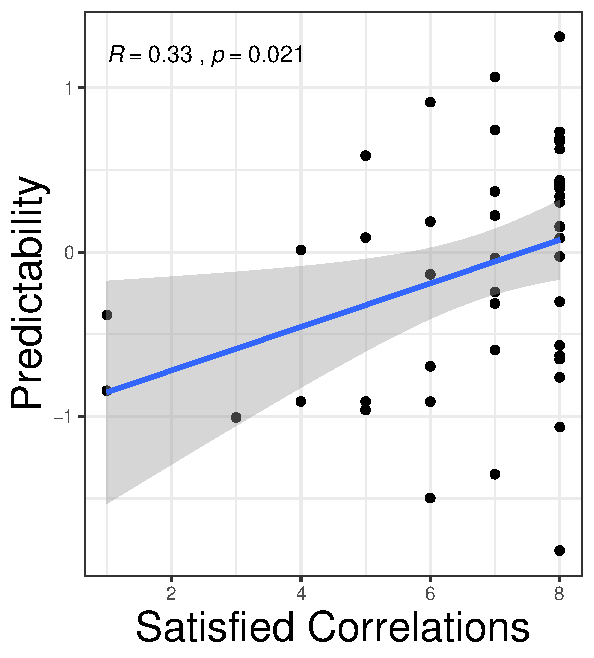
\includegraphics[scale=.25]{../results/correlations/correlations-by-grammar/ground-corrs-predictability.pdf}

	\caption{Correlation between the number of satisfied correlations ($x$-axis) and efficiency, parseability, and predictability ($y$-axis), for the 51 real languages.}
    \label{fig:todo}
\end{figure}



\section{Comparing Extracted Grammars to Linguistic Judgments}

% user@user-X510UAR:~/grammar-optim/results/grammars$ git add comparison-table.tex 

Here, we validate our grammars by comparing the dominant orders of six syntactic relations that are also annotated in WALS.
Among the eight relations that we were able to test, five are annotated in WALS.
Here, we compare our grammars with WALS on these five relations, and the verb-object relation.

WALS has some data for all but seven languages.\footnote{Note that Serbian and Croatian are listed as a single language Serbian-Croatian in WALS. In the table, we compare those with the grammar we extracted for Croatian, noting that it agrees with the Serbian grammar.}
WALS has data for 74\% of the entries, and lists a dominant order for 91\% of these.
The grammars we extracted from the corpora agree with WALS in 96~\% out of those cases where WALS records a dominant word order.

For each of the six syntactic relation, the first column provides the ordered coded in the extracted grammar; the second column provides the order coded in WALS (DH for dependent-head, HD for head-dependent order). `?' indicates that WALS has no data.
$*$ indicates that WALS does not list a dominant order, which can mean that both orders occur in the language, or that insufficient data was available when compiling WALS \citep{dryer2011evidence}.
Finally, `--' indicates that the relation does not occur in the corpus.


\small{
\begin{longtable}{l||ll|ll|ll|ll|ll|ll|llllll}
%	   for(dep in c("obj", "lifted_mark", "acl", "nmod", "obl")) {
		   Language 
		   &	\multicolumn{2}{|c|}{Objects} 
		   &	\multicolumn{2}{|c|}{Adpositions} 
		   &	\multicolumn{2}{|c|}{Compl.} 
		   &	\multicolumn{2}{|c|}{Rel.Cl.} 
		   &	\multicolumn{2}{|c|}{Genitive} 
		   &	\multicolumn{2}{|c|}{PP}  \\ \hline\hline
	Afrikaans  & DH  & ?  & HD  & ?  & HD  & ?  & --  & ?  & HD  & ?  & HD  & ?  & \\ 
Anc.Grk.  & DH  & ?  & HD  & ?  & HD  & ?  & HD  & ?  & HD  & ?  & HD  & ?  & \\ 
Arabic  & HD  & HD  & HD  & HD  & HD  & HD  & HD  & ?  & HD  & HD  & HD  & HD  & \\ 
Basque  & DH  & DH  & DH  & DH  & DH  & DH  & DH  & DH  & DH  & DH  & DH  & DH  & \\ 
Belarusian  & HD  & *  & HD  & ?  & HD  & ?  & HD  & HD  & HD  & HD  & HD  & *  & \\ 
Bulgarian  & HD  & HD  & HD  & HD  & HD  & HD  & HD  & HD  & HD  & *  & HD  & HD  & \\ 
Catalan  & HD  & HD  & HD  & HD  & HD  & ?  & HD  & HD  & HD  & HD  & HD  & ?  & \\ 
Chinese  & HD  & HD  & HD  & *  & DH  & ?  & DH  & DH  & DH  & DH  & DH  & DH  & \\ 
Coptic  & HD  & HD  & HD  & HD  & HD  & HD  & HD  & HD  & HD  & HD  & HD  & HD  & \\ 
Croatian  & HD  & HD  & HD  & HD  & HD  & HD  & HD  & ?  & HD  & *  & HD  & ?  & \\ 
Czech  & HD  & HD  & HD  & HD  & HD  & HD  & HD  & HD  & HD  & *  & HD  & ?  & \\ 
Danish  & HD  & HD  & HD  & HD  & HD  & HD  & HD  & HD  & \textit{HD} & DH  & HD  & HD  & \\ 
Dutch  & DH  & *  & HD  & HD  & HD  & HD  & HD  & HD  & HD  & HD  & DH  & *  & \\ 
English  & HD  & HD  & HD  & HD  & HD  & HD  & HD  & HD  & HD  & *  & HD  & HD  & \\ 
Estonian  & HD  & HD  & DH  & DH  & HD  & HD  & \textit{DH} & HD  & DH  & DH  & HD  & HD  & \\ 
Finnish  & HD  & HD  & DH  & DH  & HD  & HD  & \textit{DH} & HD  & DH  & DH  & HD  & HD  & \\ 
French  & HD  & HD  & HD  & HD  & HD  & HD  & HD  & HD  & HD  & HD  & HD  & HD  & \\ 
Galician  & HD  & ?  & HD  & ?  & HD  & ?  & HD  & ?  & HD  & ?  & HD  & ?  & \\ 
German  & HD  & *  & HD  & HD  & HD  & HD  & HD  & HD  & HD  & HD  & DH  & *  & \\ 
Gothic  & HD  & ?  & HD  & ?  & HD  & ?  & HD  & ?  & HD  & ?  & HD  & ?  & \\ 
Greek  & HD  & HD  & HD  & HD  & HD  & HD  & HD  & HD  & HD  & HD  & HD  & ?  & \\ 
Hebrew  & HD  & HD  & HD  & HD  & HD  & HD  & HD  & HD  & HD  & HD  & HD  & ?  & \\ 
Hindi  & DH  & DH  & DH  & DH  & HD  & HD  & DH  & *  & DH  & DH  & DH  & ?  & \\ 
Hungarian  & \textit{DH} & HD  & DH  & DH  & HD  & HD  & HD  & *  & DH  & DH  & DH  & ?  & \\ 
Indonesian  & HD  & HD  & HD  & HD  & HD  & HD  & HD  & HD  & HD  & HD  & HD  & HD  & \\ 
Irish  & HD  & HD  & HD  & HD  & HD  & HD  & HD  & HD  & HD  & HD  & HD  & HD  & \\ 
Italian  & HD  & HD  & HD  & HD  & HD  & HD  & HD  & HD  & HD  & HD  & HD  & ?  & \\ 
Japanese  & DH  & DH  & DH  & DH  & DH  & DH  & DH  & DH  & DH  & DH  & DH  & DH  & \\ 
Korean  & DH  & DH  & DH  & DH  & \textit{HD} & DH  & DH  & DH  & DH  & DH  & DH  & ?  & \\ 
Latin  & DH  & ?  & HD  & ?  & HD  & ?  & HD  & ?  & HD  & ?  & DH  & ?  & \\ 
Latvian  & HD  & HD  & HD  & HD  & HD  & HD  & HD  & HD  & DH  & DH  & DH  & ?  & \\ 
Lithuanian  & HD  & HD  & HD  & HD  & HD  & HD  & HD  & HD  & DH  & DH  & DH  & ?  & \\ 
Marathi  & DH  & DH  & DH  & DH  & HD  & *  & DH  & DH  & DH  & DH  & DH  & ?  & \\ 
Norwegian  & HD  & HD  & HD  & HD  & HD  & HD  & HD  & HD  & HD  & *  & HD  & ?  & \\ 
O.C.Slav.  & HD  & ?  & HD  & ?  & HD  & ?  & HD  & ?  & HD  & ?  & HD  & ?  & \\ 
Persian  & DH  & DH  & HD  & HD  & HD  & HD  & HD  & HD  & HD  & HD  & DH  & ?  & \\ 
Polish  & HD  & HD  & HD  & HD  & HD  & HD  & HD  & HD  & HD  & HD  & HD  & ?  & \\ 
Portuguese  & HD  & HD  & HD  & HD  & HD  & ?  & HD  & HD  & HD  & HD  & HD  & ?  & \\ 
Romanian  & HD  & HD  & HD  & HD  & HD  & HD  & HD  & HD  & HD  & HD  & HD  & ?  & \\ 
Russian  & HD  & HD  & HD  & HD  & HD  & HD  & HD  & HD  & HD  & HD  & HD  & ?  & \\ 
Serbian  & HD  & ?  & HD  & ?  & HD  & ?  & HD  & ?  & HD  & ?  & HD  & ?  & \\ 
Slovak  & HD  & ?  & HD  & ?  & HD  & ?  & HD  & ?  & HD  & ?  & HD  & ?  & \\ 
Slovenian  & HD  & HD  & HD  & HD  & HD  & ?  & HD  & ?  & HD  & *  & HD  & ?  & \\ 
Spanish  & HD  & HD  & HD  & HD  & HD  & HD  & HD  & HD  & HD  & HD  & HD  & HD  & \\ 
Swedish  & HD  & HD  & HD  & HD  & HD  & HD  & HD  & HD  & \textit{HD} & DH  & HD  & HD  & \\ 
Tamil  & DH  & DH  & DH  & DH  & DH  & *  & \textit{HD} & DH  & DH  & DH  & DH  & DH  & \\ 
Telugu  & DH  & DH  & DH  & DH  & DH  & *  & DH  & DH  & DH  & DH  & DH  & ?  & \\ 
Turkish  & DH  & DH  & DH  & DH  & DH  & *  & DH  & DH  & DH  & DH  & DH  & DH  & \\ 
Ukrainian  & HD  & HD  & HD  & HD  & HD  & HD  & HD  & HD  & HD  & ?  & HD  & ?  & \\ 
Urdu  & DH  & DH  & DH  & DH  & HD  & HD  & HD  & *  & DH  & DH  & DH  & ?  & \\ 
Vietnamese  & HD  & HD  & HD  & HD  & \textit{DH} & HD  & --  & HD  & HD  & HD  & HD  & HD  & \\ 

\end{longtable}
}




\bibliographystyle{unsrtnat}
\bibliography{everything}


\end{document}
